\section{Der Würfel} % (fold)
\label{sec:the_cube}
\subsection*{}

\begin{frame}
	\frametitle{Geschichte}

	\begin{itemize}
		\item Erfunden 1975 vom ungarischen Architekten Ern\H o Rubik
		\item Sonderpreis als \glqq Spiel des Jahres\grqq{} 1980
		\item Die durchschnittliche optimale Lösung benötigt 18 Züge (Richard Korf, 1997)
		\item Es werden (für die optimale Lösung) nie mehr als 22 Züge benötigt (Tomas Rokicki, 2008)
		\item Aktueller 3$\times$3$\times$3 Weltrekord: 7,08 Sek. (Erik Akkersdijk, 13.~Juli 2008)
	\end{itemize}
	
\end{frame}

\begin{frame}
	\frametitle{Mittelstücke}
	
	\begin{columns}[c]
		\begin{column}[C]{.5\textwidth}
			\center
			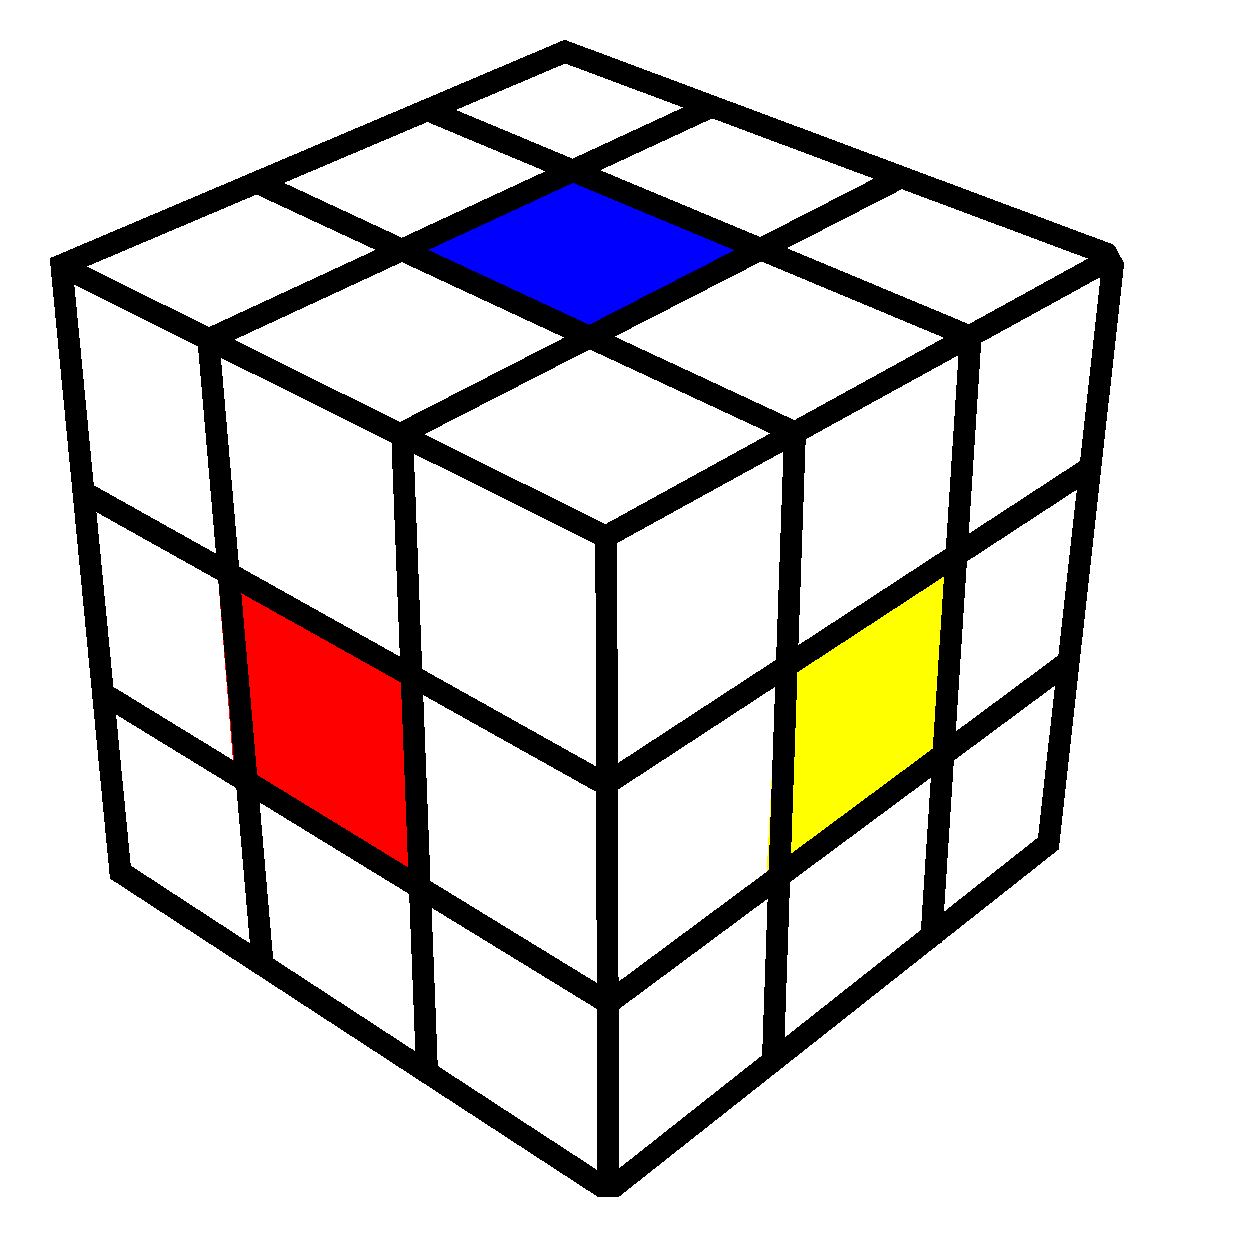
\includegraphics[scale=0.3]{img/middles}
		\end{column}
		\begin{column}[C]{.5\textwidth}
			\begin{itemize}
				\item bleiben (beim 3$\times$3$\times$3\,-\,Würfel) immer an ihrer Stelle
				\item geben die Farbe der Seite an
			\end{itemize}
		\end{column}
	\end{columns}	
	
\end{frame}

\begin{frame}
	\frametitle{Kanten}
	
	\begin{columns}[c]
		\begin{column}[C]{.5\textwidth}
			\center
			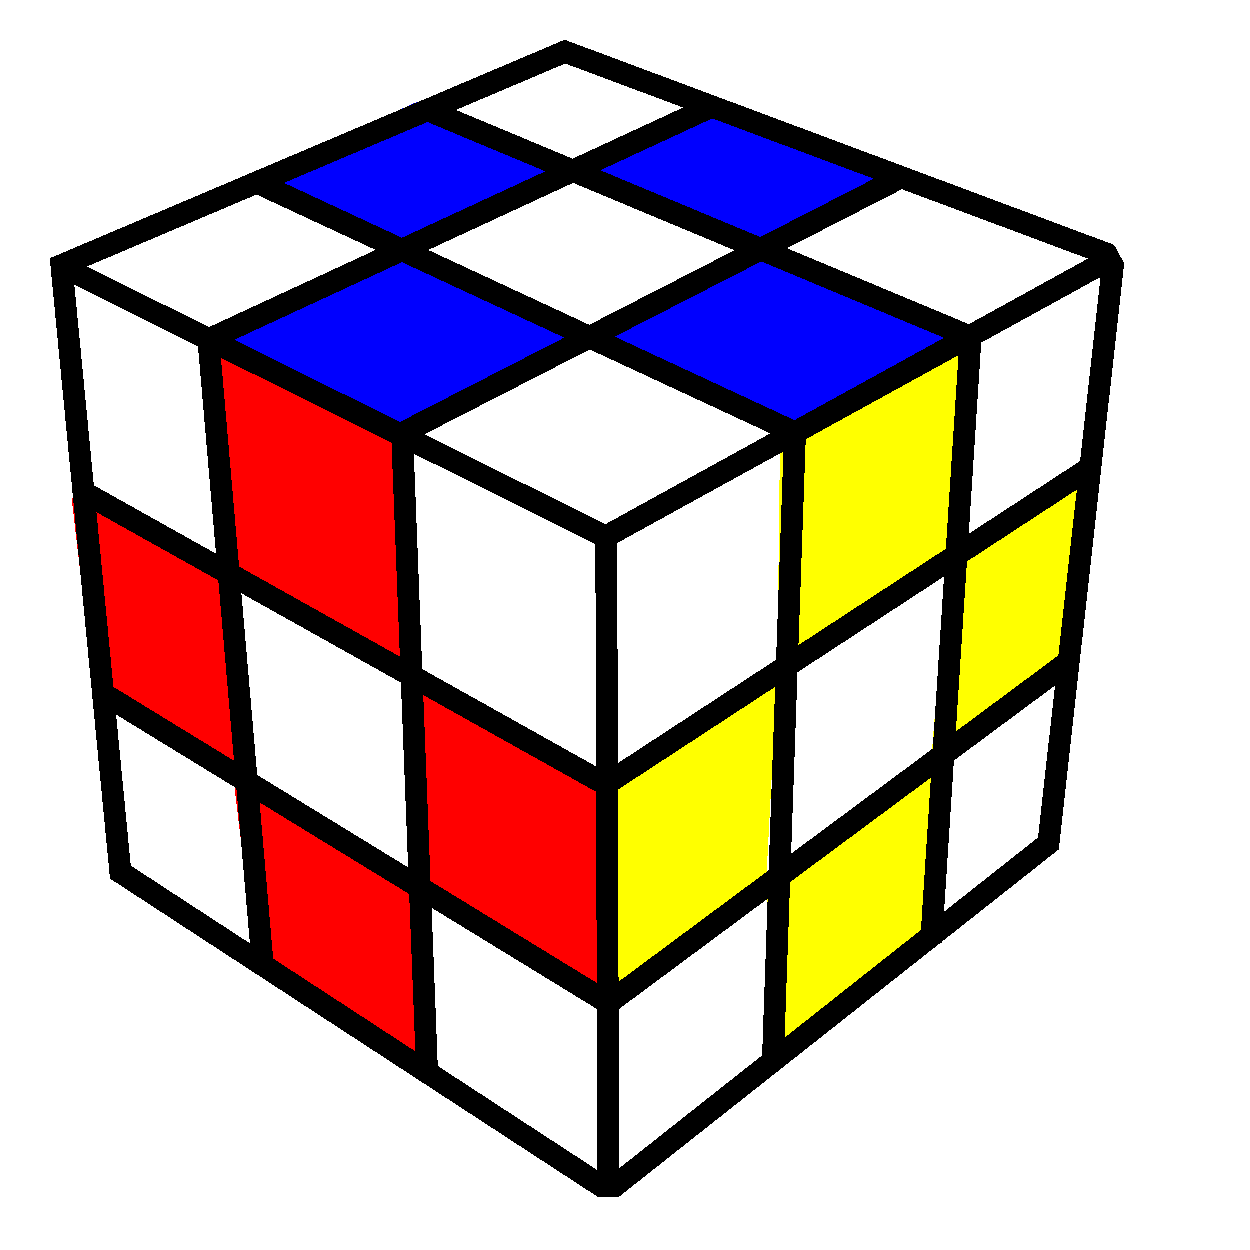
\includegraphics[scale=0.3]{img/nodes}
		\end{column}
		\begin{column}[C]{.5\textwidth}
			\begin{itemize}
				\item müssen an zwei Seiten ausgerichtet werden
				\item können an 12 verschiedenen Positionen sein
				\item es gibt keine Kanten für gegenüberliegende Farben
			\end{itemize}
		\end{column}
	\end{columns}	
	
\end{frame}

\begin{frame}
	\frametitle{Ecken}
	
	\begin{columns}[c]
		\begin{column}[C]{.5\textwidth}
			\center
			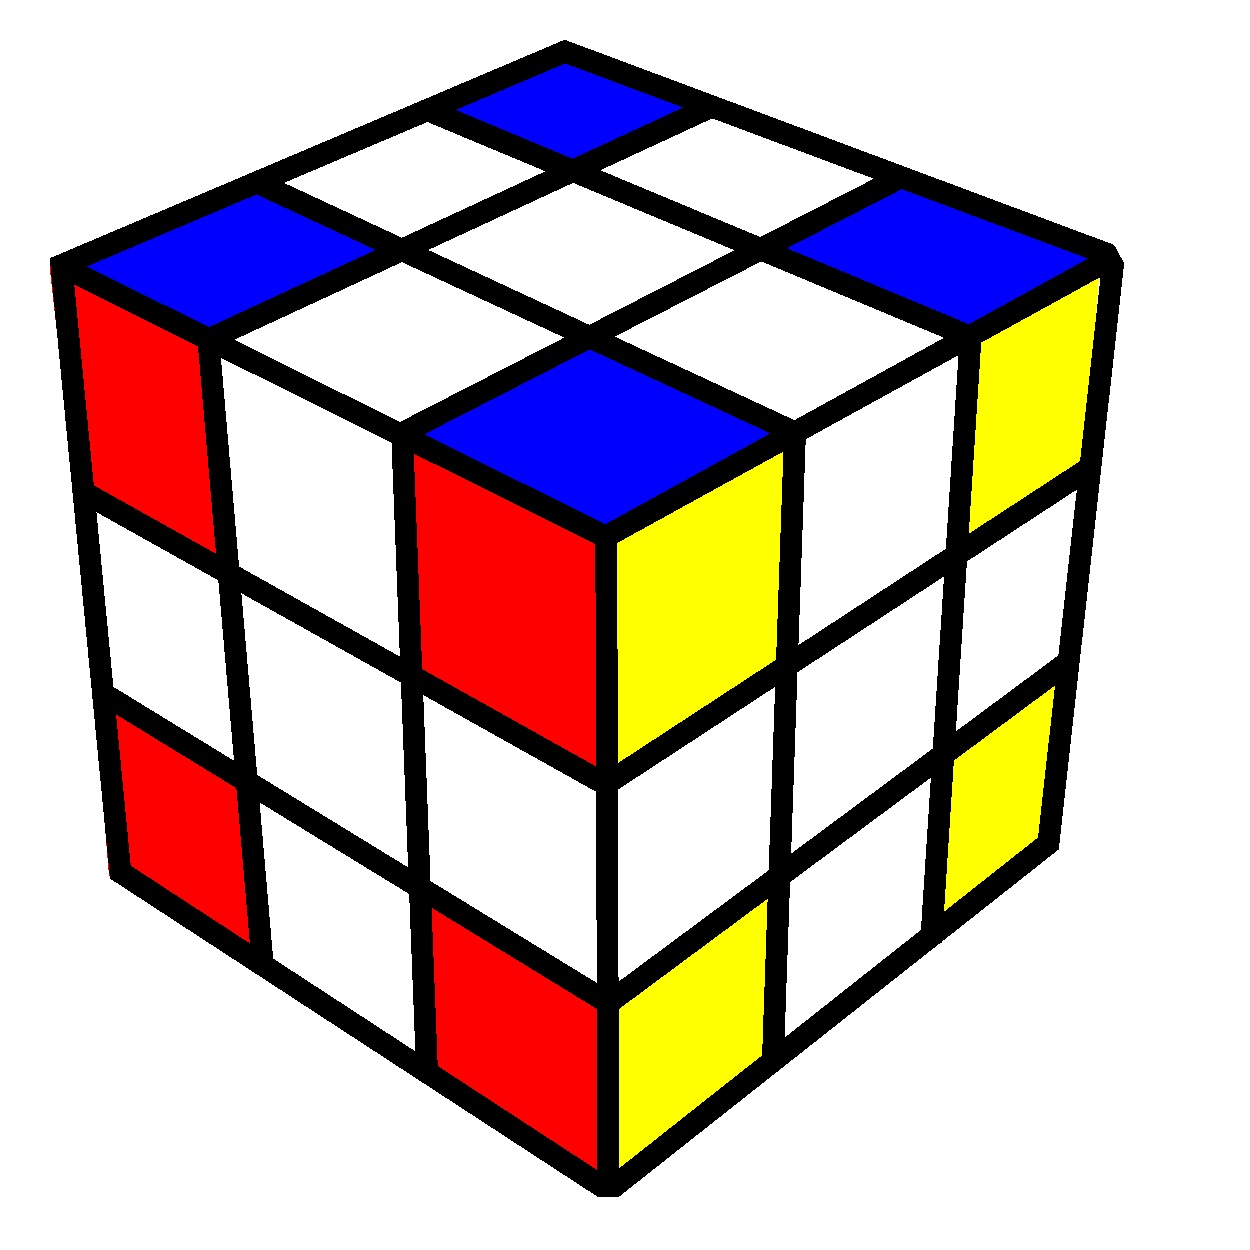
\includegraphics[scale=0.3]{img/edges}
		\end{column}
		\begin{column}[C]{.5\textwidth}
			\begin{itemize}
				\item müssen an drei Seiten ausgerichtet werden
				\item können an 8 verschiedenen Positionen sein
			\end{itemize}
		\end{column}
	\end{columns}	
	
\end{frame}

\begin{frame}
	\frametitle{Seiten}

	\begin{columns}[c]
		\begin{column}[C]{.8\textwidth}
			\center
			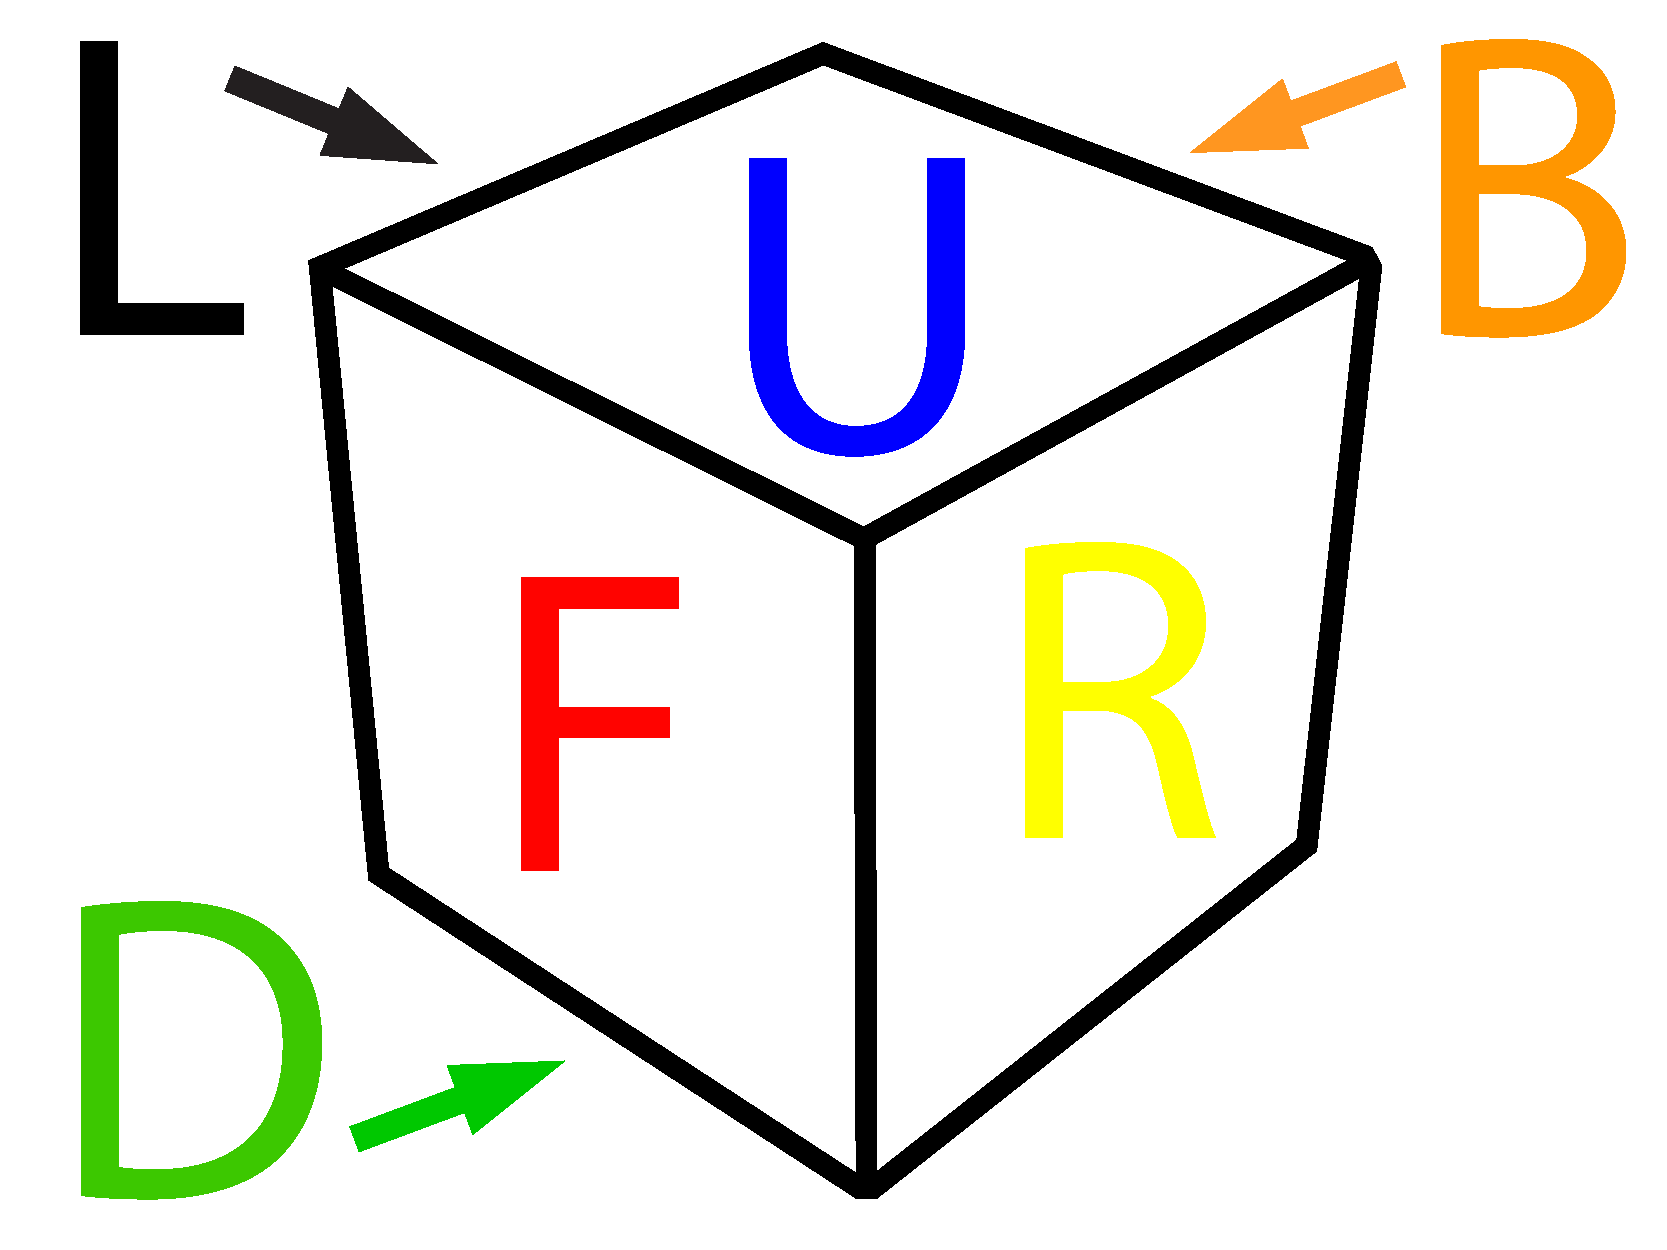
\includegraphics[scale=0.3]{img/sides}
		\end{column}
		\begin{column}[C]{.2\textwidth}
			\begin{itemize}
				\item \textbf{\underline{U}}p
				\item \textbf{\underline{D}}own
				\item \textbf{\underline{L}}eft
				\item \textbf{\underline{R}}ight
				\item \textbf{\underline{F}}ront
				\item \textbf{\underline{B}}ack
			\end{itemize}
		\end{column}
	\end{columns}
	
\end{frame}

\begin{frame}
	\frametitle{Notation}
	
	\begin{block}{$X$}
		Drehung der Seite $X$ um 90\gradneu{} im Uhrzeigersinn
	\end{block}
	
	\begin{block}{$X^2$}
		Drehung der Seite $X$ um 180\gradneu{} im Uhrzeigersinn
	\end{block}
	
	\begin{block}{$X^{-1}$}
		Drehung der Seite $X$ um 90\gradneu{} gegen den Uhrzeigersinn
	\end{block}
	
	\begin{exampleblock}{Beispiel}
		$R^{-1}D^{-1}RD \,\Rightarrow$ \glqq Right inverted, down inverted, right, down\grqq
	\end{exampleblock}
	
	\begin{exampleblock}{Alternative Schreibweisen}
		$\overline{R}\,\overline{D}RD$ ; $r\,d\,R\,D$ ; $Ri\,Di\,R\,D$
	\end{exampleblock}
	
\end{frame}

% section the_cube (end)


\section{Ebene 1} % (fold)
\label{sec:ebene_1}

\subsection*{}

\begin{frame}
	\frametitle{Das Kreuz}
	
	\begin{columns}[c]
		\begin{column}[C]{.5\textwidth}
			\center
			\only<1>{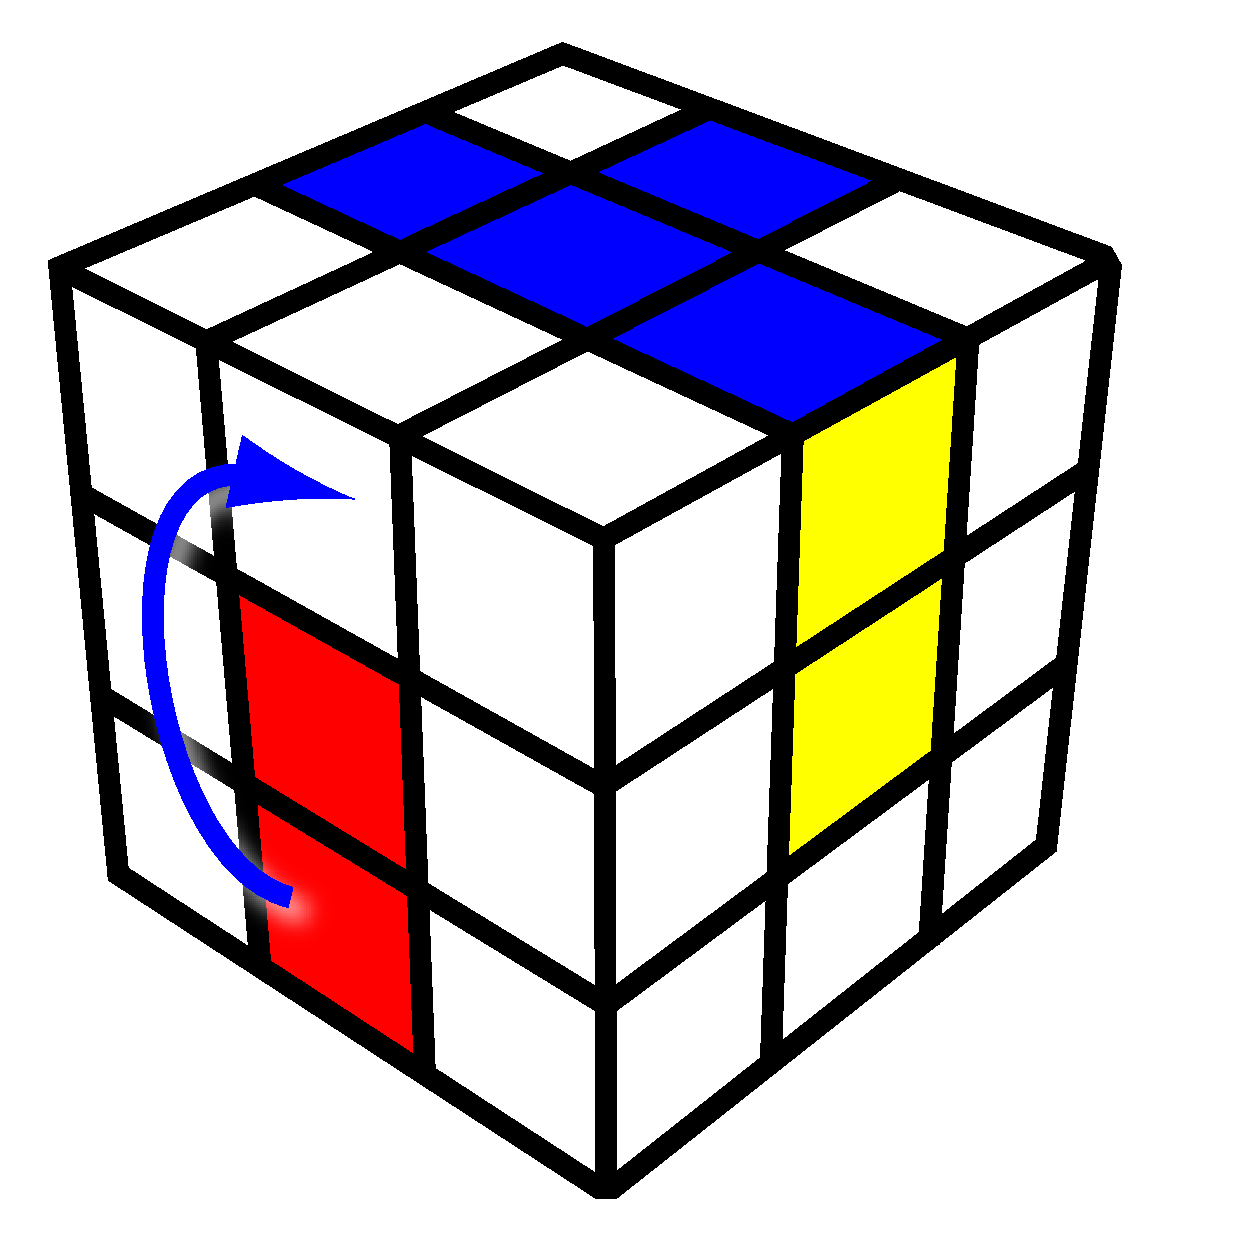
\includegraphics[scale=0.3]{img/cross1}}
			\only<2>{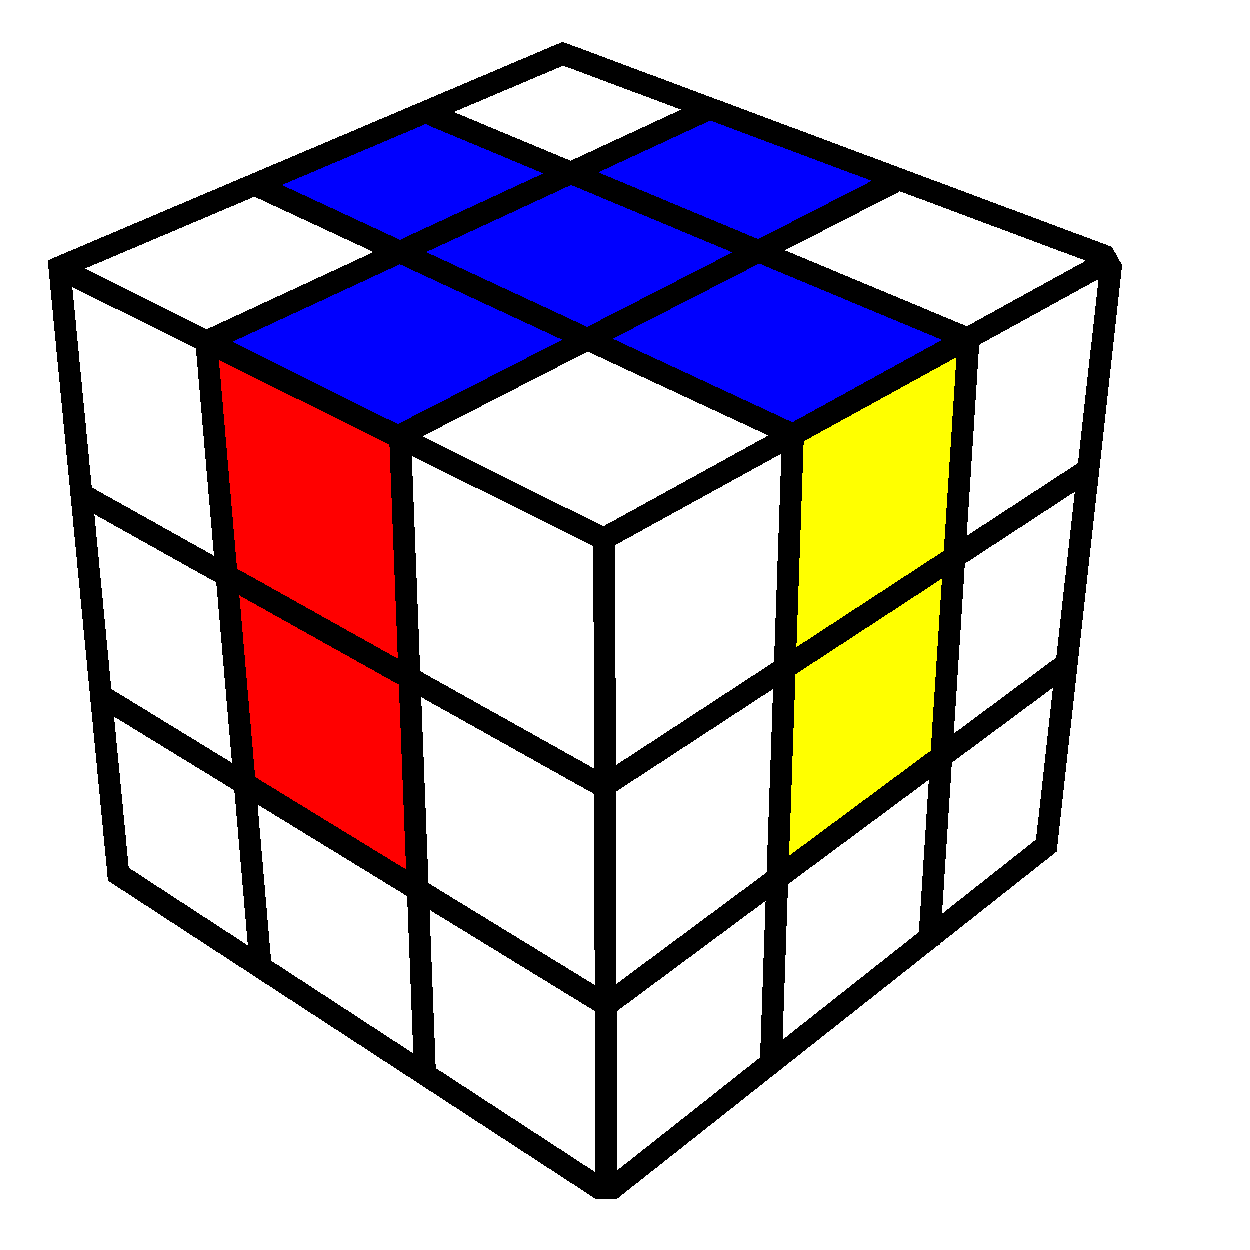
\includegraphics[scale=0.3]{img/cross2}}
		\end{column}
		\begin{column}[C]{.5\textwidth}
			\begin{block}{Ziel}
				Ein Kreuz auf der Oberseite.
			\end{block}
			\begin{exampleblock}{Algorithmus}
				Kante \glqq unter\grqq{} die gewünschte Stelle bringen und durch $F^2$ an die richtige Position drehen.
			\end{exampleblock}
			\begin{alertblock}{Wichtig}
				Die Kanten zu den anliegenden Seiten müssen übereinstimmen!
			\end{alertblock}
		\end{column}
	\end{columns}
	
\end{frame}

\begin{frame}
	\frametitle{Kanten drehen}
	
	\begin{columns}[c]
		\begin{column}[C]{.5\textwidth}
			\center
			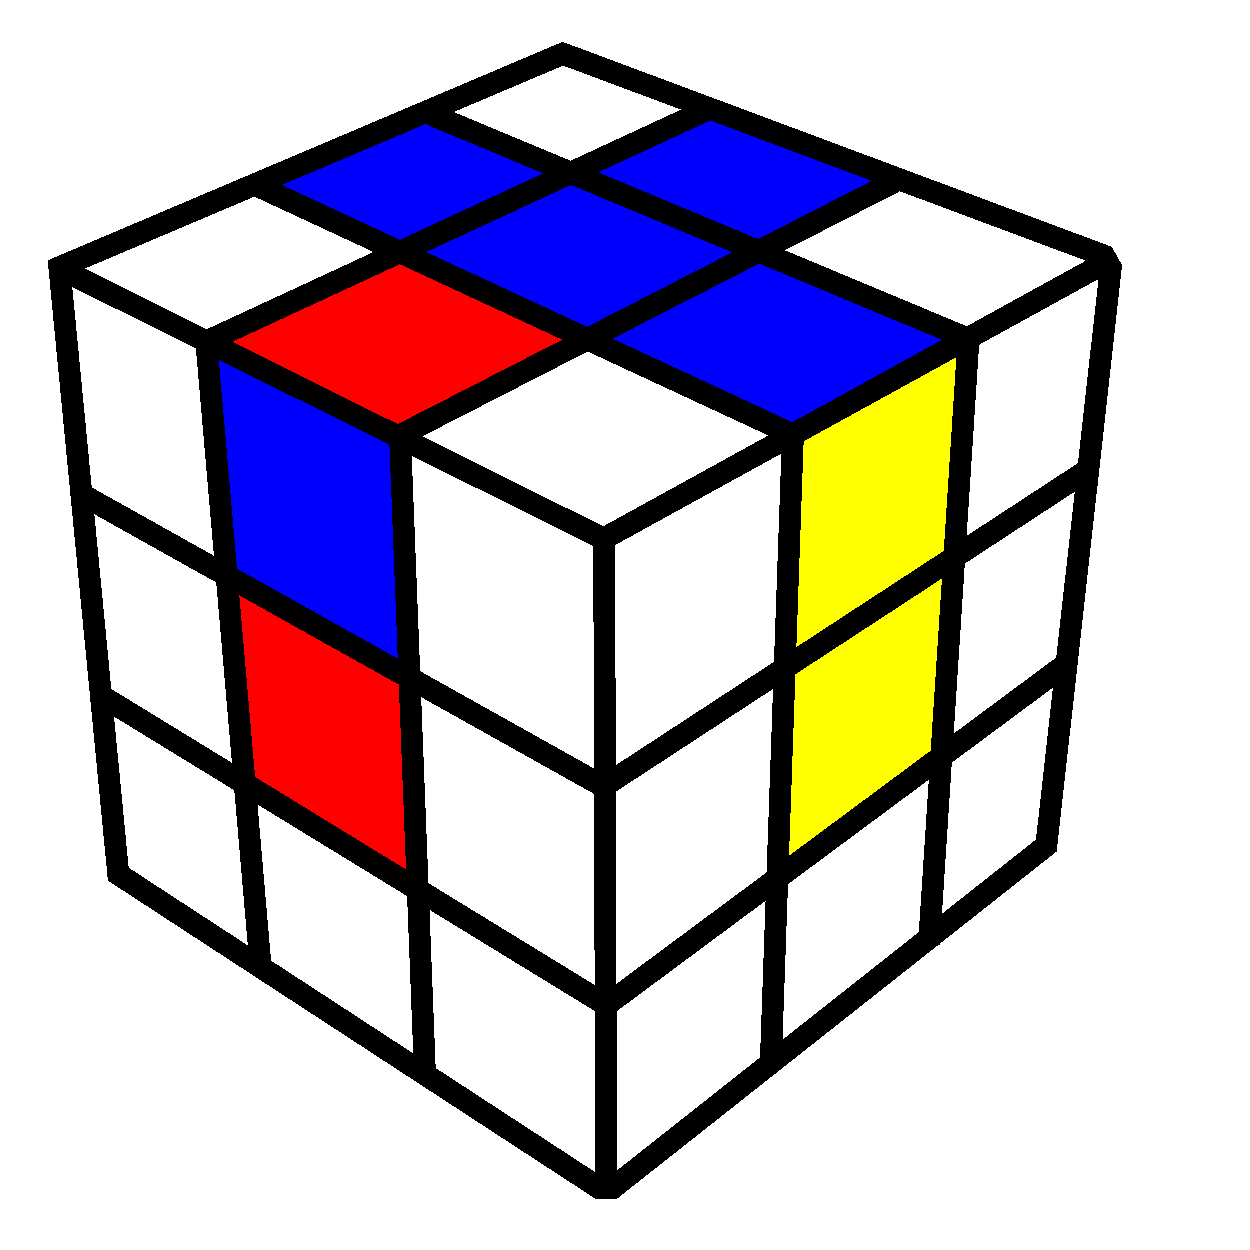
\includegraphics[scale=0.3]{img/nodeflip}
		\end{column}
		\begin{column}[C]{.5\textwidth}
			\begin{alertblock}{Problem}
				Die Kante ist um 180\gradneu{} gedreht.
			\end{alertblock}
			\begin{exampleblock}{Algorithmus}
				$F^{-1}UL^{-1}U^{-1}$
			\end{exampleblock}
		\end{column}
	\end{columns}
	
\end{frame}

\begin{frame}
	\frametitle{Die Ecken}
	
	\begin{columns}[c]
		\begin{column}[C]{.5\textwidth}
			\center
			\only<1>{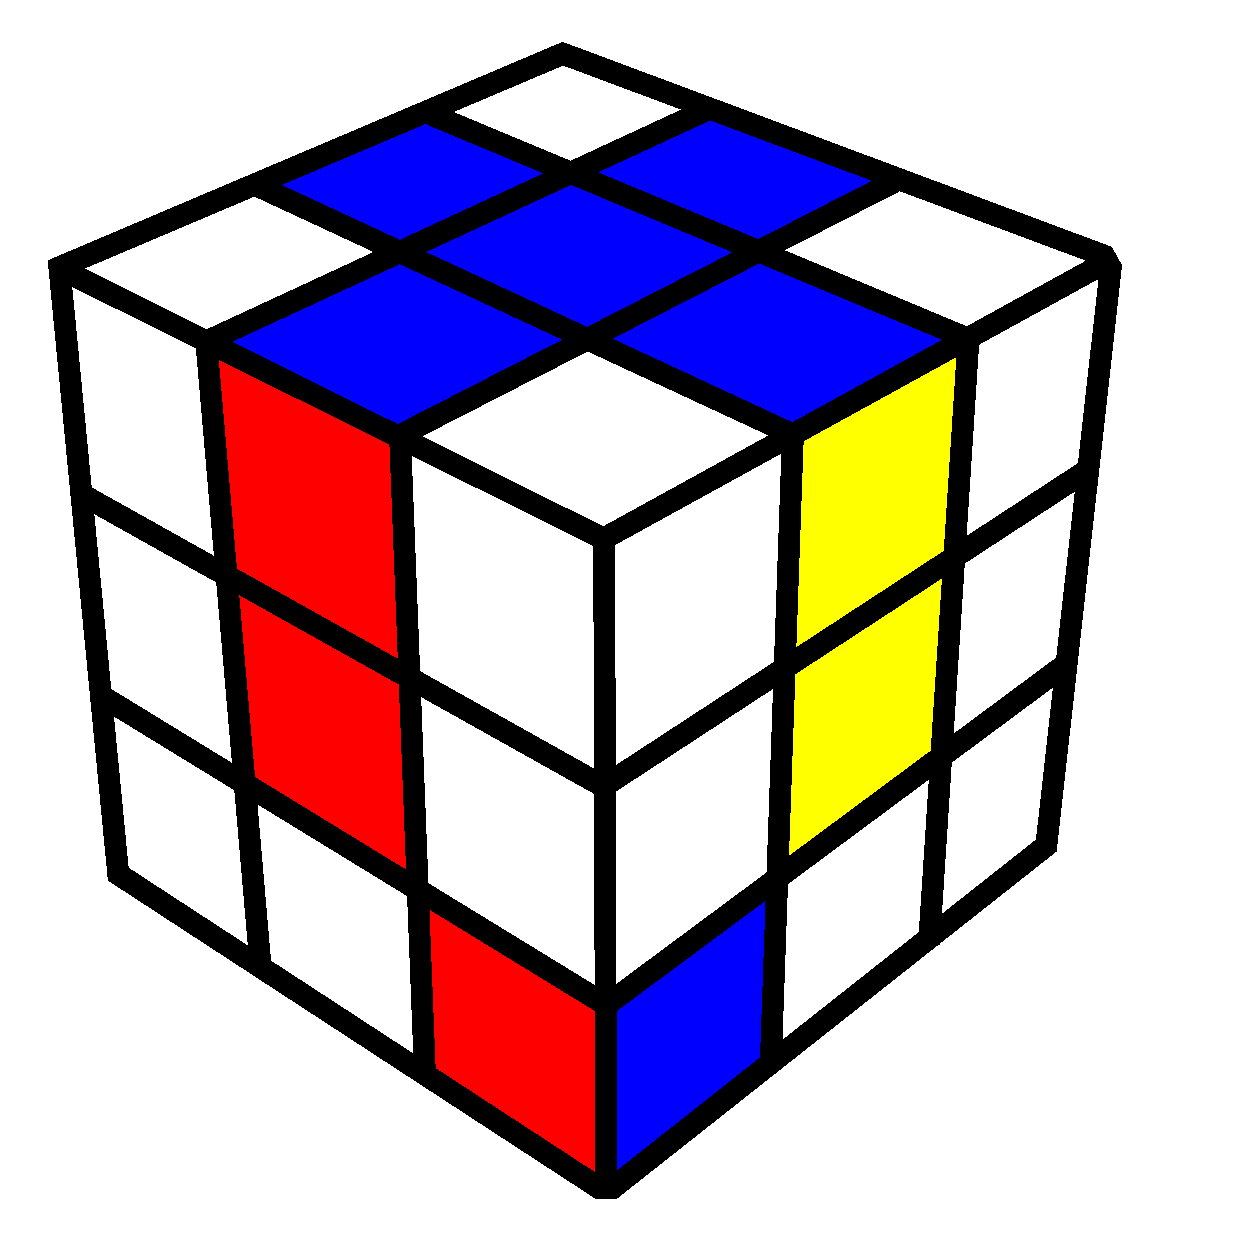
\includegraphics[scale=0.3]{img/layer1edge1}}
			\only<2->{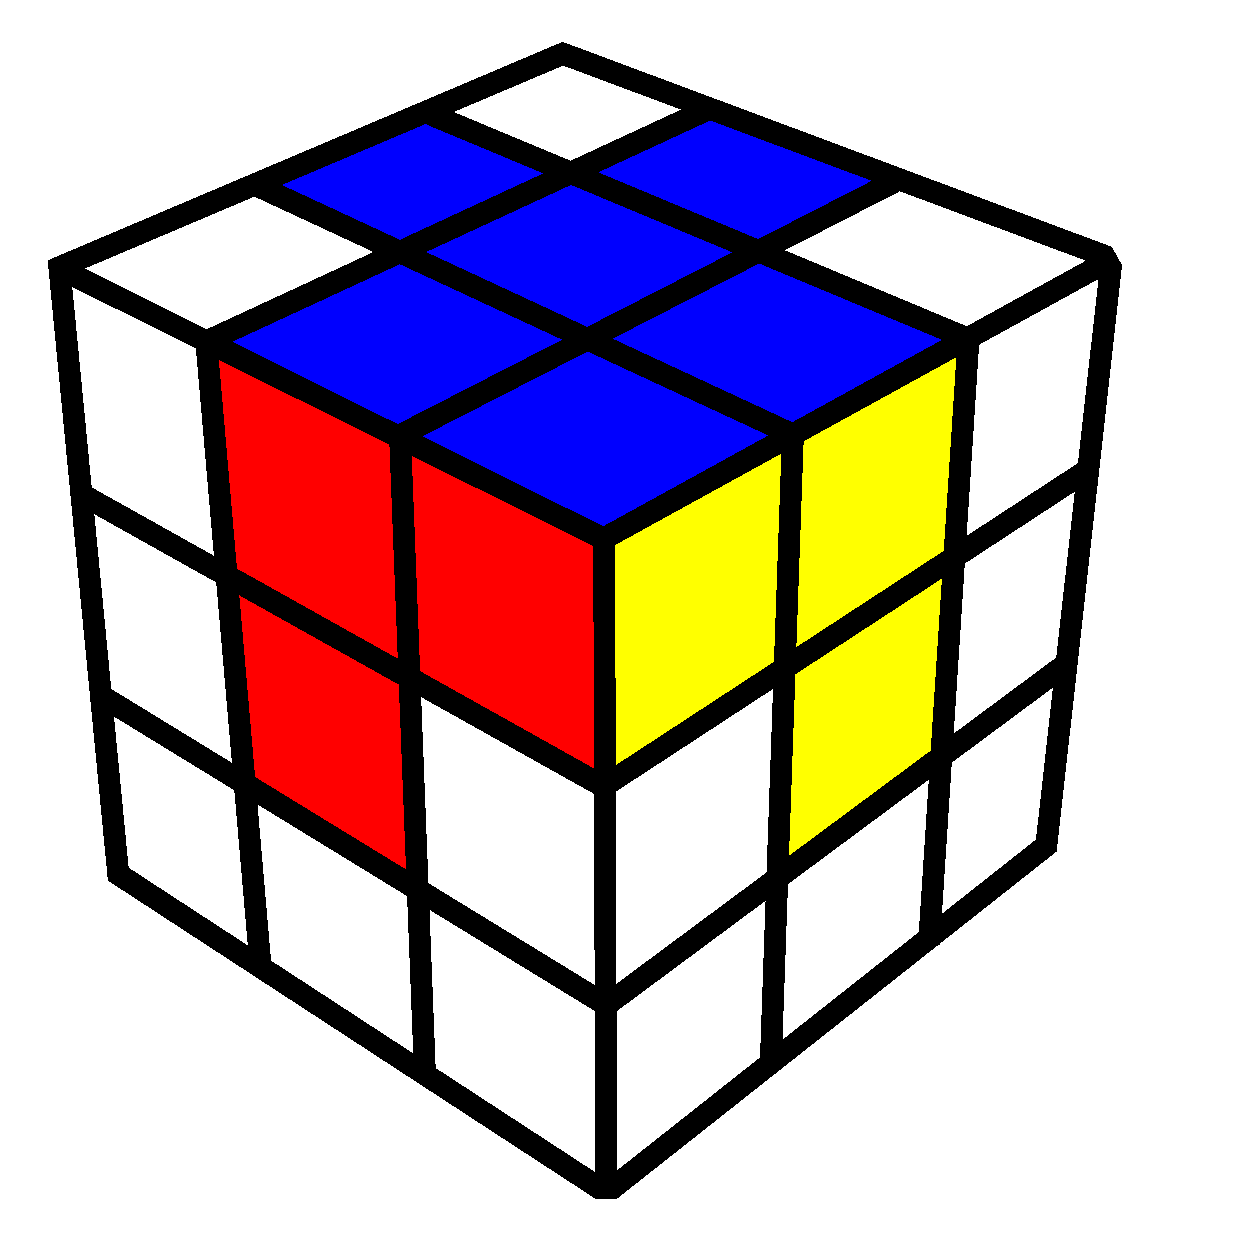
\includegraphics[scale=0.3]{img/layer1edge2}}
		\end{column}
		\begin{column}[C]{.5\textwidth}
			\begin{block}{Ziel}
				Ebene 1 durch Platzierung der Ecken fertigstellen.
			\end{block}
			\begin{exampleblock}{Algorithmus}
				Ecke \glqq unter\grqq{} die gewünschte Stelle bringen und durch (ggf. mehrfaches Anwenden von) $R^{-1}D^{-1}RD$ positionieren.
			\end{exampleblock}
			\begin{alertblock}{Wichtig}
				Die Farben der drei Seiten des Ecksteins (hier: blau, rot und gelb) müssen beachtet werden!
			\end{alertblock}
		\end{column}
	\end{columns}
	
\end{frame}

\begin{frame}
	\frametitle{Ebene 1 ist fertig!}
	
	\begin{columns}[c]
		\begin{column}[C]{.5\textwidth}
			\center
			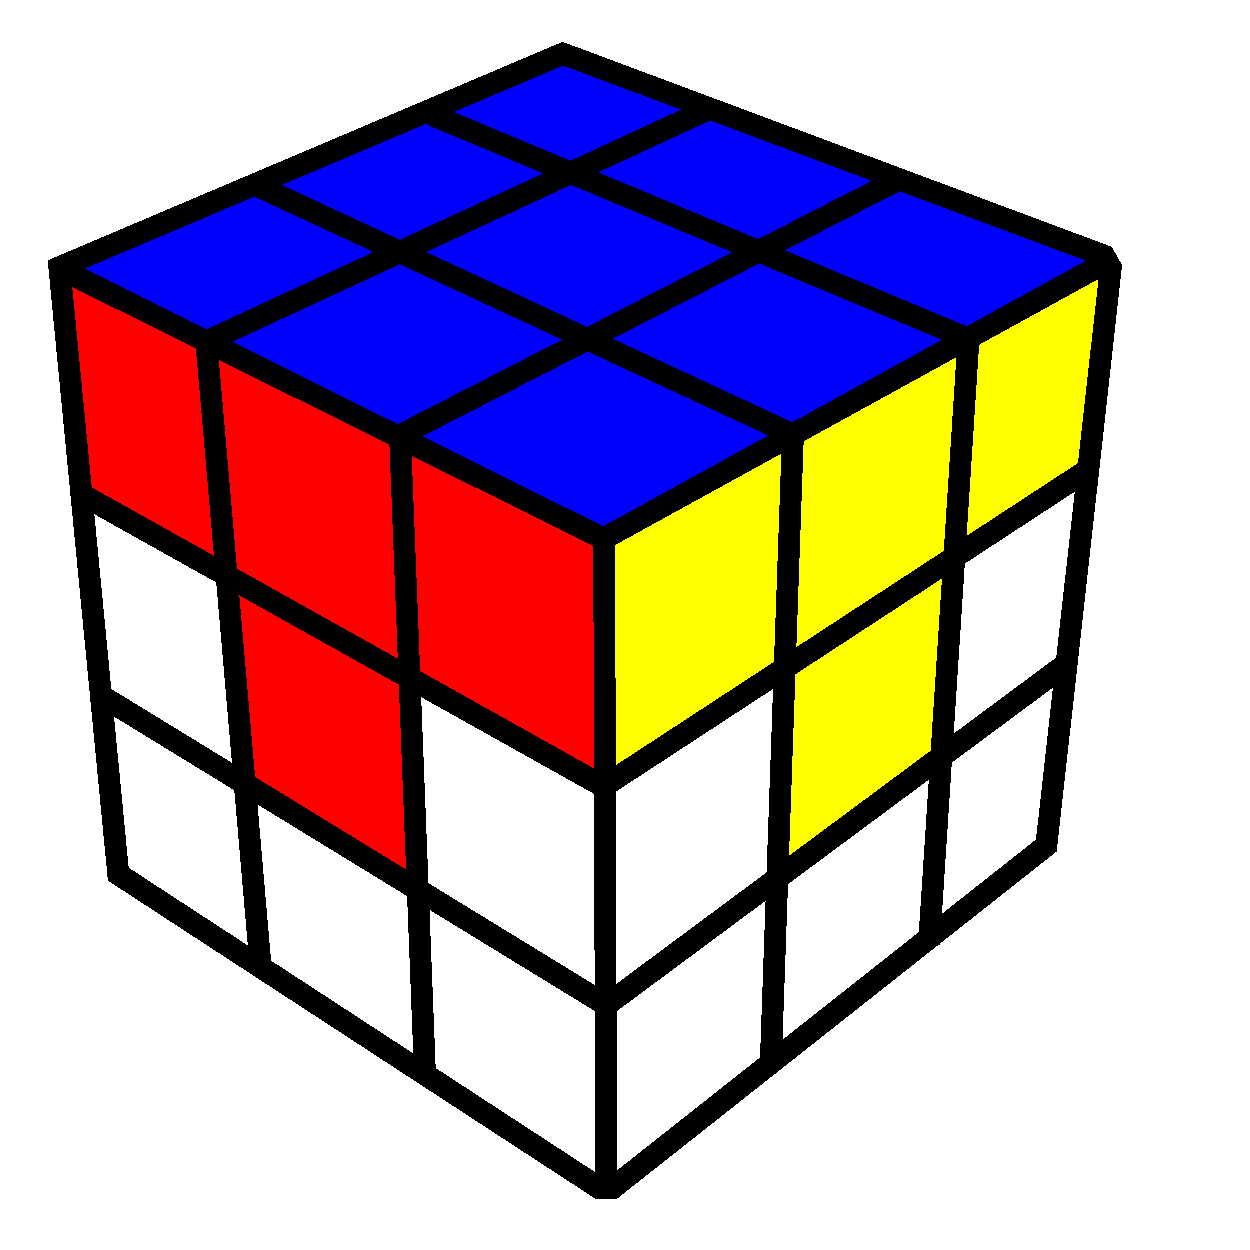
\includegraphics[scale=0.3]{img/layer1edge3}
		\end{column}
		\begin{column}[C]{.5\textwidth}
			\begin{itemize}
				\item Würfel bereits zu 40\% gelöst!
				\item Für das weitere Vorgehen wird der Würfel um $180^\circ$ gedreht -- die blaue Seite zeigt nun nach unten.
			\end{itemize}
		\end{column}
	\end{columns}
	
\end{frame}

% section ebene_1 (end)


\section{Ebene 2} % (fold)
\label{sec:ebene_2}

\subsection*{}

\begin{frame}
	\frametitle{Vier Kanten -- Möglichkeit 1}
	
	\begin{columns}[c]
		\begin{column}[C]{.5\textwidth}
			\center
			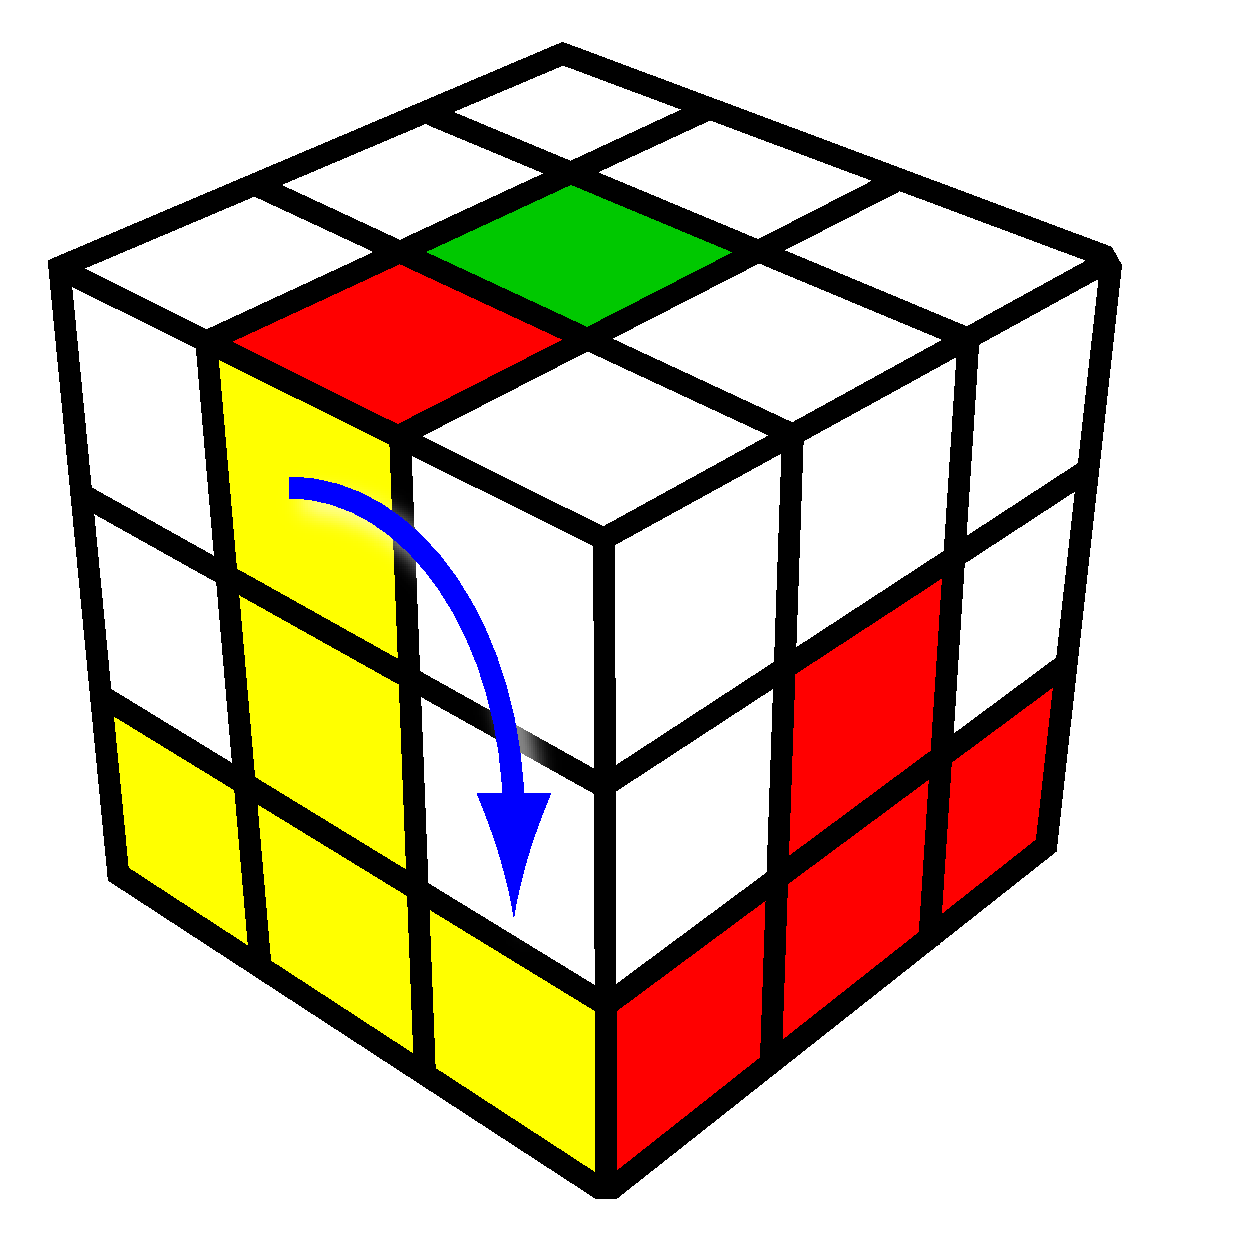
\includegraphics[scale=0.3]{img/layer2edge1}
		\end{column}
		\begin{column}[C]{.5\textwidth}
			\begin{block}{Ziel}
				Passende Kante aus Ebene 3 (oben) in Ebene 2 bringen.
			\end{block}
			\begin{exampleblock}{Algorithmus}
				Kante oben mittig platzieren und durch $URU^{-1}R^{-1}U^{-1}F^{-1}UF$ nach rechts kippen.
			\end{exampleblock}
		\end{column}
	\end{columns}
	
\end{frame}

\begin{frame}
	\frametitle{Vier Kanten -- Möglichkeit 2}
	
	\begin{columns}[c]
		\begin{column}[C]{.5\textwidth}
			\center
			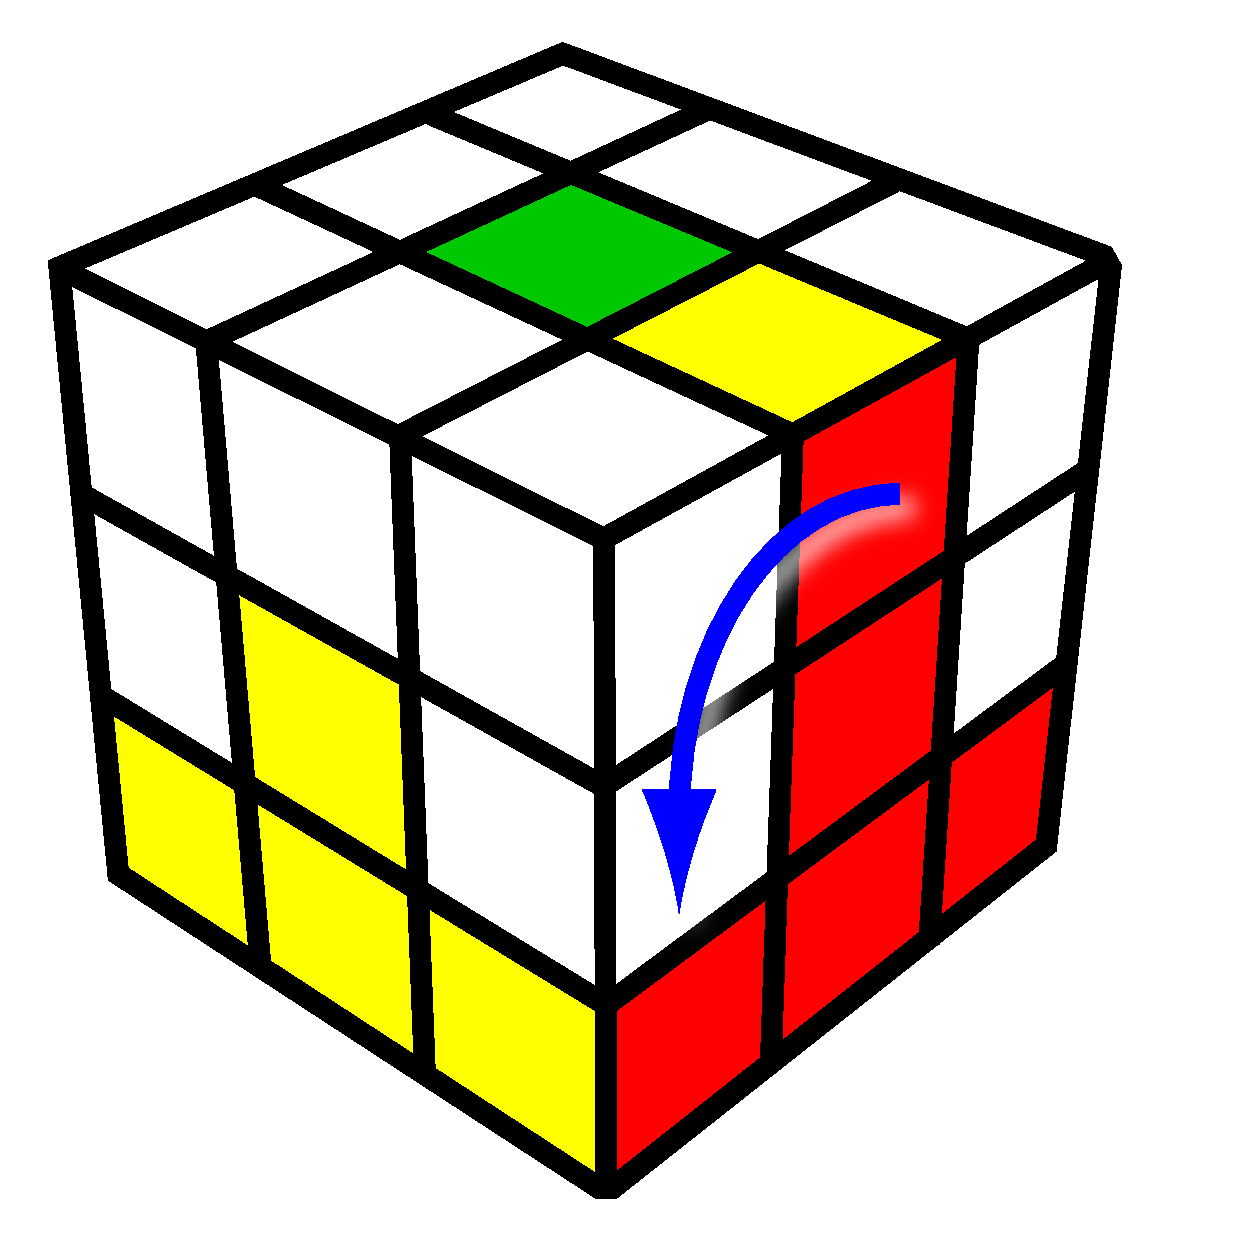
\includegraphics[scale=0.3]{img/layer2edge2}			
		\end{column}
		\begin{column}[C]{.5\textwidth}
			\begin{block}{Ziel}
				Passende Kante aus Ebene 3 (oben) in Ebene 2 bringen.
			\end{block}
			\begin{exampleblock}{Algorithmus}
				Kante oben mittig platzieren und durch $U^{-1}L^{-1}ULUFU^{-1}F^{-1}$ nach links kippen.
			\end{exampleblock}
		\end{column}
	\end{columns}
	
\end{frame}

\begin{frame}
	\frametitle{Vier Kanten -- Algorithmenübersicht}
	
	\begin{columns}[c]
		\begin{column}[C]{.5\textwidth}
			\center
			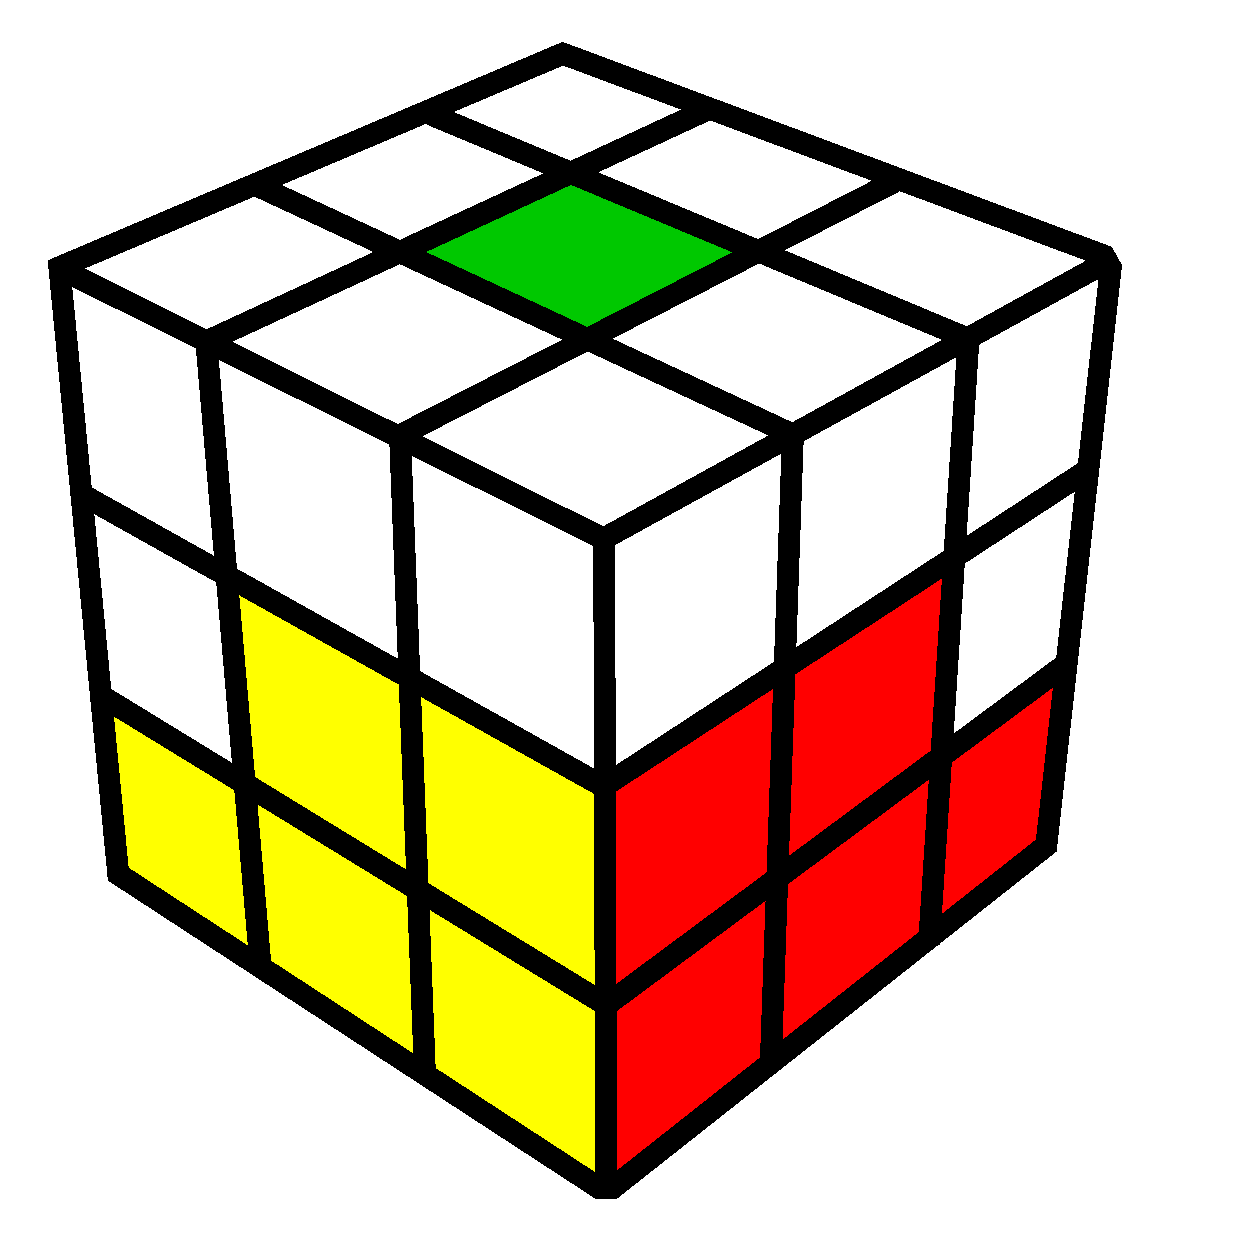
\includegraphics[scale=0.3]{img/layer2edge3}
		\end{column}
		\begin{column}[C]{.5\textwidth}
			\begin{exampleblock}{Algorithmus 1}
				Kante oben mittig platzieren und durch $URU^{-1}R^{-1}U^{-1}F^{-1}UF$ nach rechts kippen.
			\end{exampleblock}
			\begin{exampleblock}{Algorithmus 2}
				Kante oben mittig platzieren und durch $U^{-1}L^{-1}ULUFU^{-1}F^{-1}$ nach links kippen.
			\end{exampleblock}
		\end{column}
	\end{columns}
	
\end{frame}

\begin{frame}
	\frametitle{Ebene 2 ist fertig!}
	
	\begin{columns}[c]
		\begin{column}[C]{.5\textwidth}
			\center
			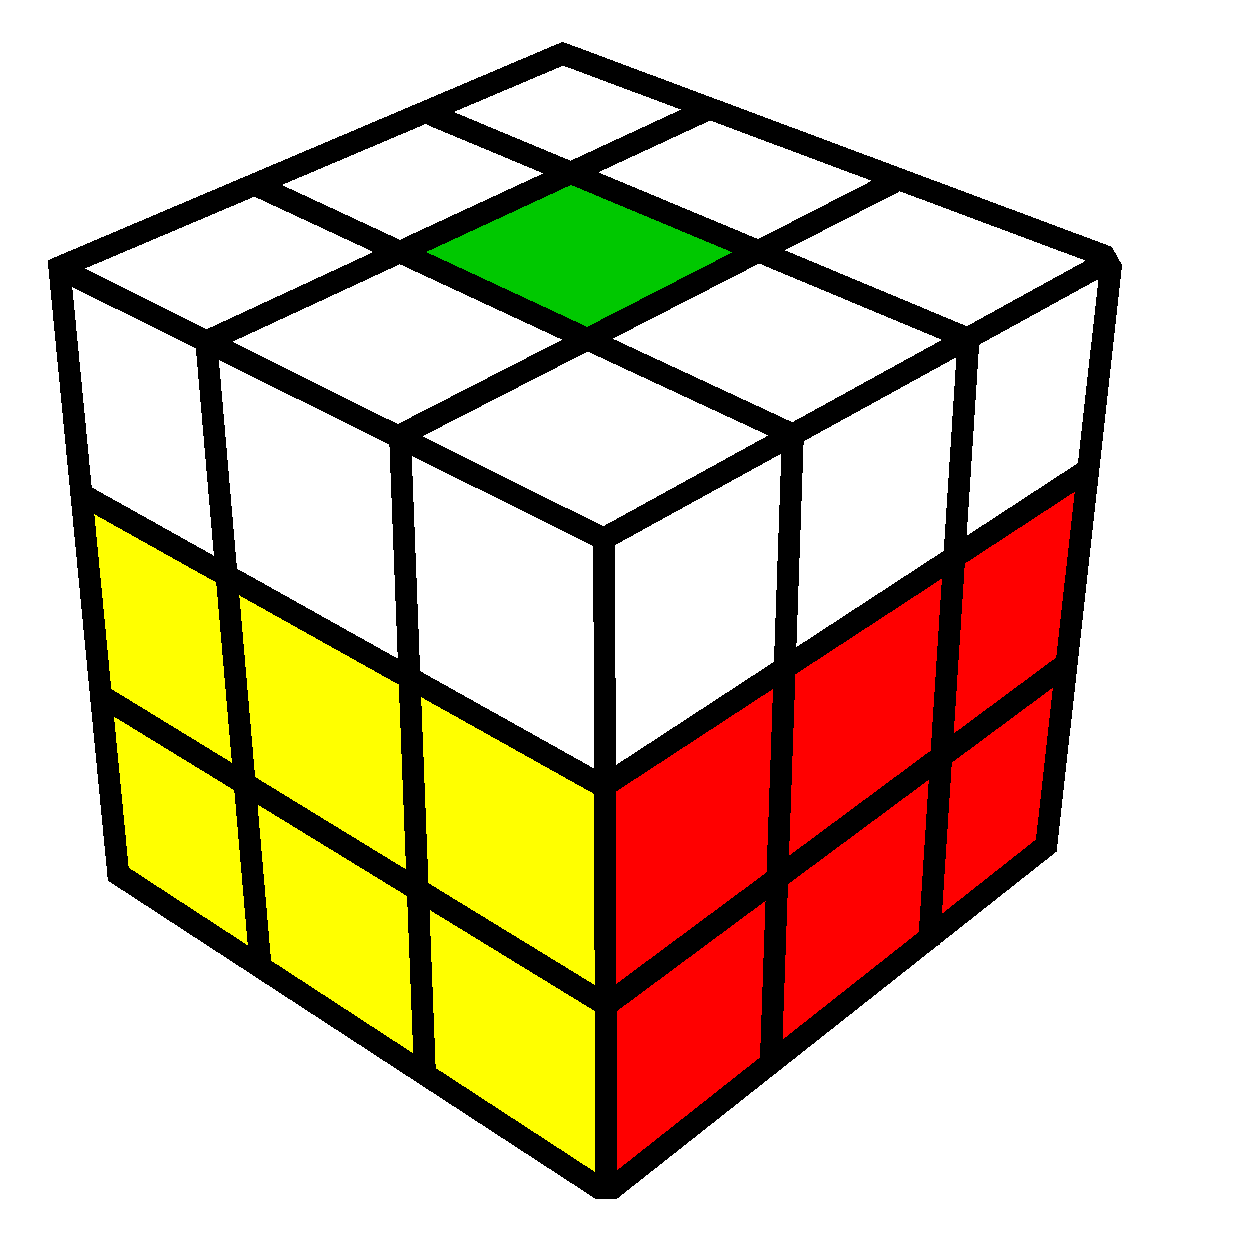
\includegraphics[scale=0.3]{img/layer2edge4}
		\end{column}
		\begin{column}[C]{.5\textwidth}
			\begin{itemize}
				\item Würfel jetzt schon zu 60\% gelöst!
				\item Ebene 3 wird ein klein wenig komplizierter...
			\end{itemize}
		\end{column}
	\end{columns}
	
\end{frame}

% section ebene_2 (end)


\section{Ebene 3} % (fold)
\label{sec:ebene_3}

\subsection*{}

\begin{frame}
	\frametitle{Wieder ein Kreuz -- Situation 1}
	
	\begin{columns}[c]
		\begin{column}[C]{.5\textwidth}
			\center
			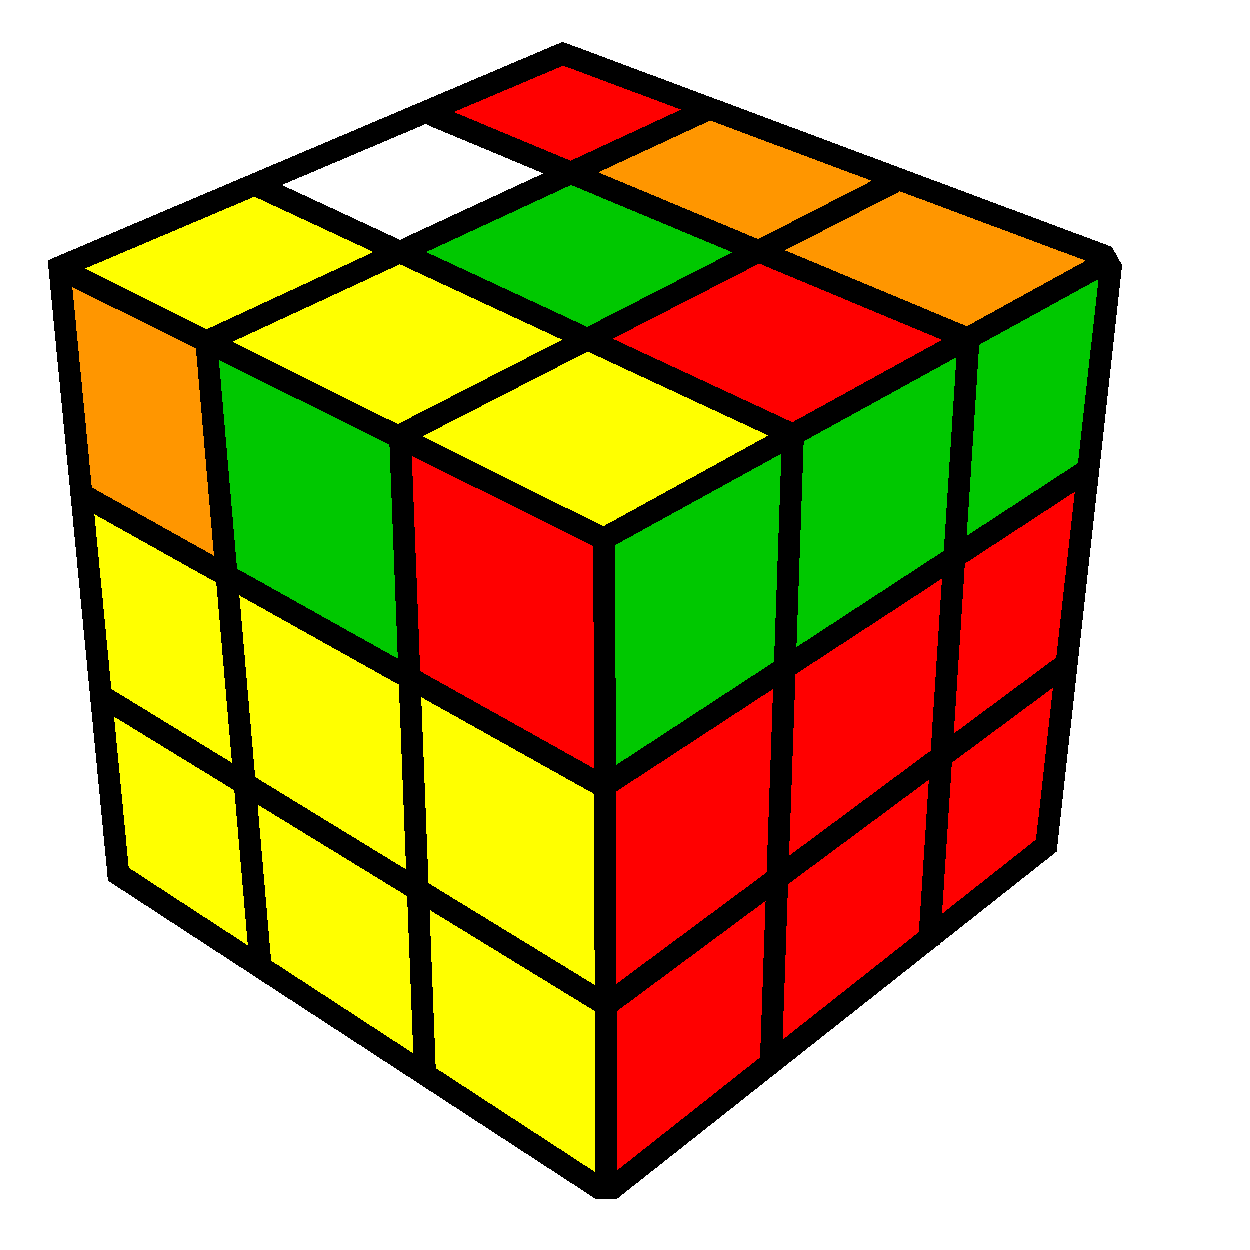
\includegraphics[scale=0.3]{img/layer3nothing}
		\end{column}
		\begin{column}[C]{.5\textwidth}
			\begin{block}{Ziel}
				L-förmige Anordnung von Steinen der Farbe der Oberseite ($\rightarrow$~Situation 2).
			\end{block}
			\begin{exampleblock}{Algorithmus}
				$FRUR^{-1}U^{-1}F^{-1}$
			\end{exampleblock}
		\end{column}
	\end{columns}
	
\end{frame}

\begin{frame}
	\frametitle{Wieder ein Kreuz -- Situation 2}
	
	\begin{columns}[c]
		\begin{column}[C]{.5\textwidth}
			\center
			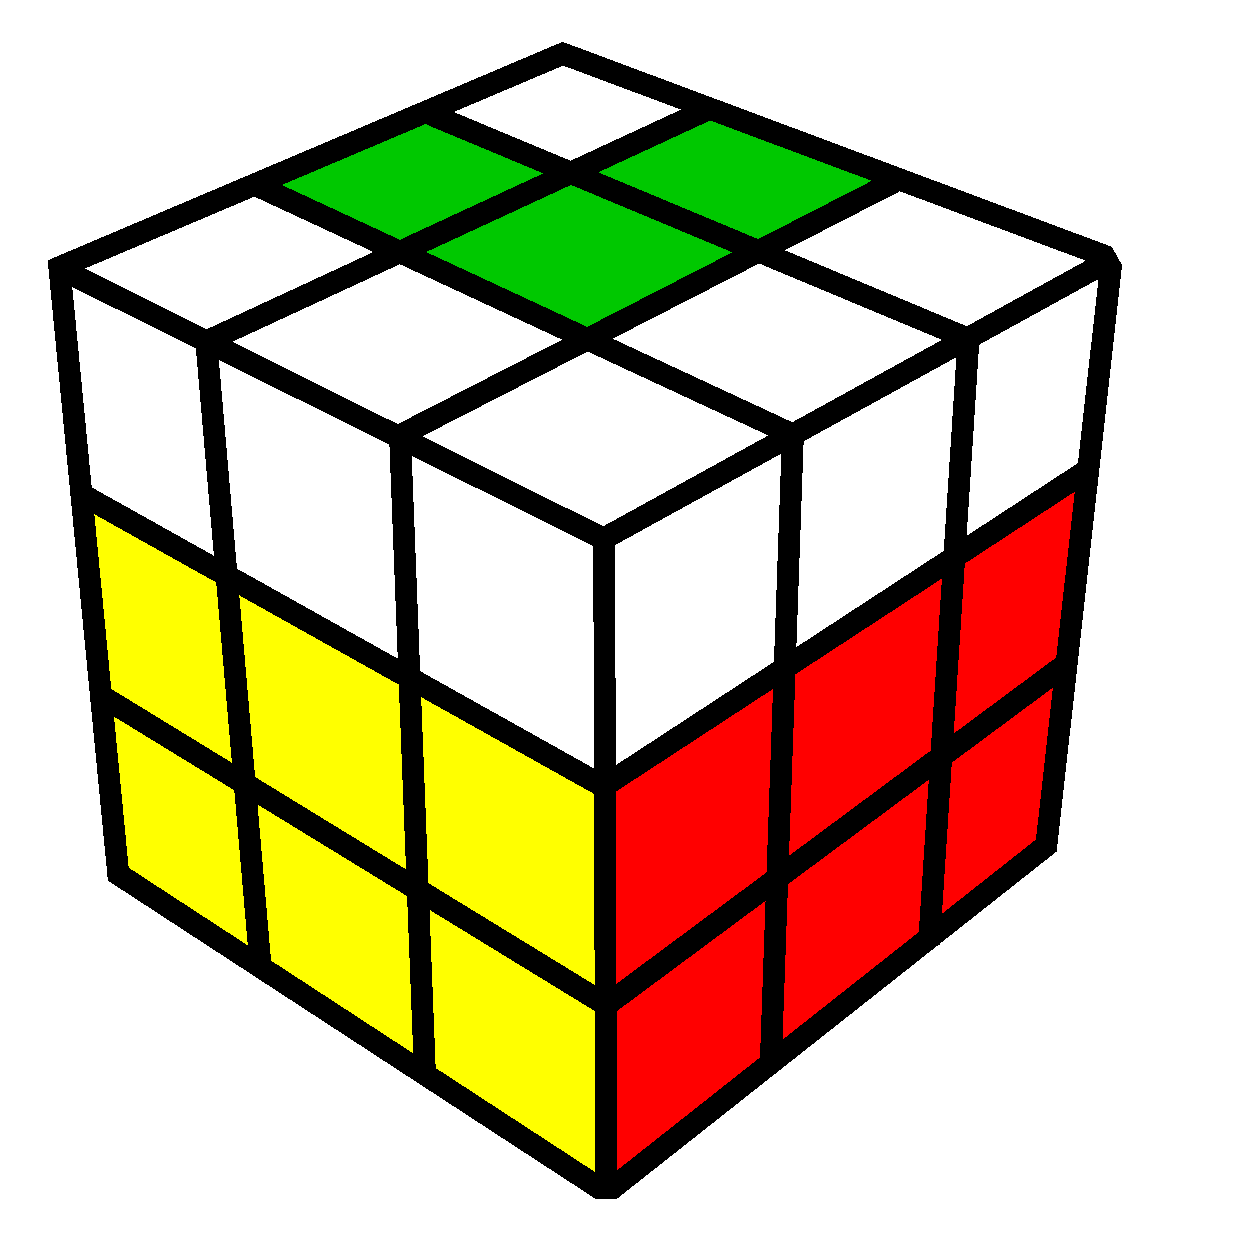
\includegraphics[scale=0.3]{img/layer3L}
		\end{column}
		\begin{column}[C]{.5\textwidth}
			\begin{block}{Ziel}
				Drei Steine in der Farbe der Oberseite in einer Reihe ($\rightarrow$~Situation 3).
			\end{block}
			\begin{exampleblock}{Algorithmus}
				$FRUR^{-1}U^{-1}F^{-1}$
			\end{exampleblock}
			\begin{alertblock}{Wichtig}
				Der Würfel muss so gehalten werden, dass sich das \glqq L\grqq{} in der oberen linken Ecke befindet.
			\end{alertblock}
		\end{column}
	\end{columns}
	
\end{frame}

\begin{frame}
	\frametitle{Wieder ein Kreuz -- Situation 3}
	
	\begin{columns}[c]
		\begin{column}[C]{.5\textwidth}
			\center
			\only<1>{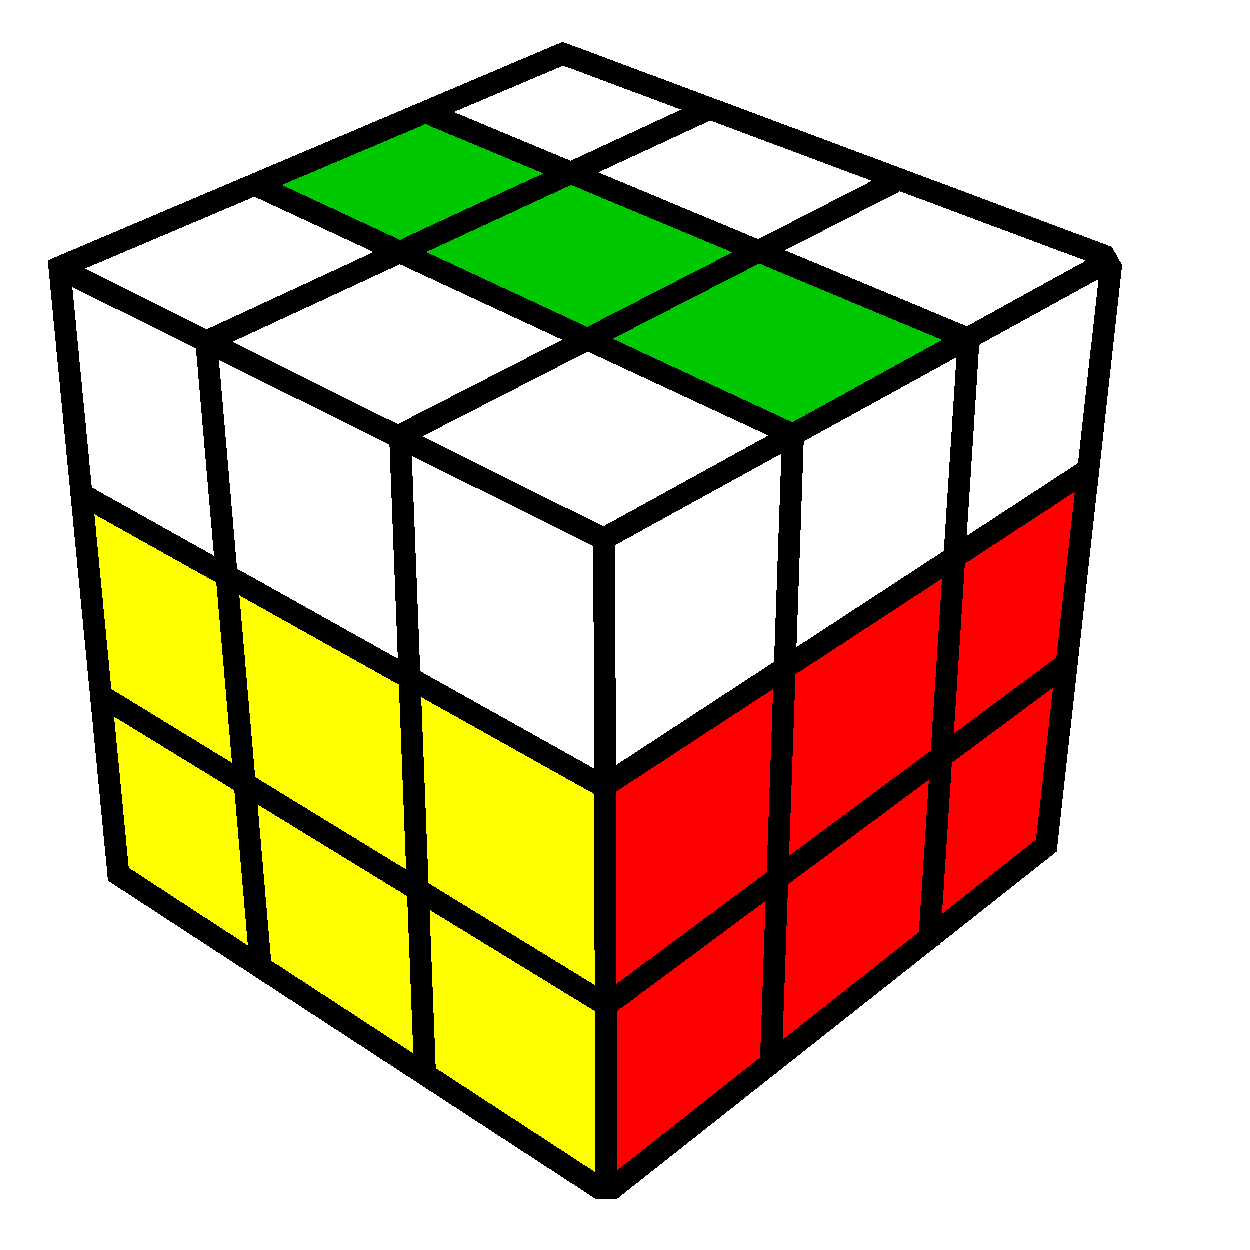
\includegraphics[scale=0.3]{img/layer3line}}
			\only<2>{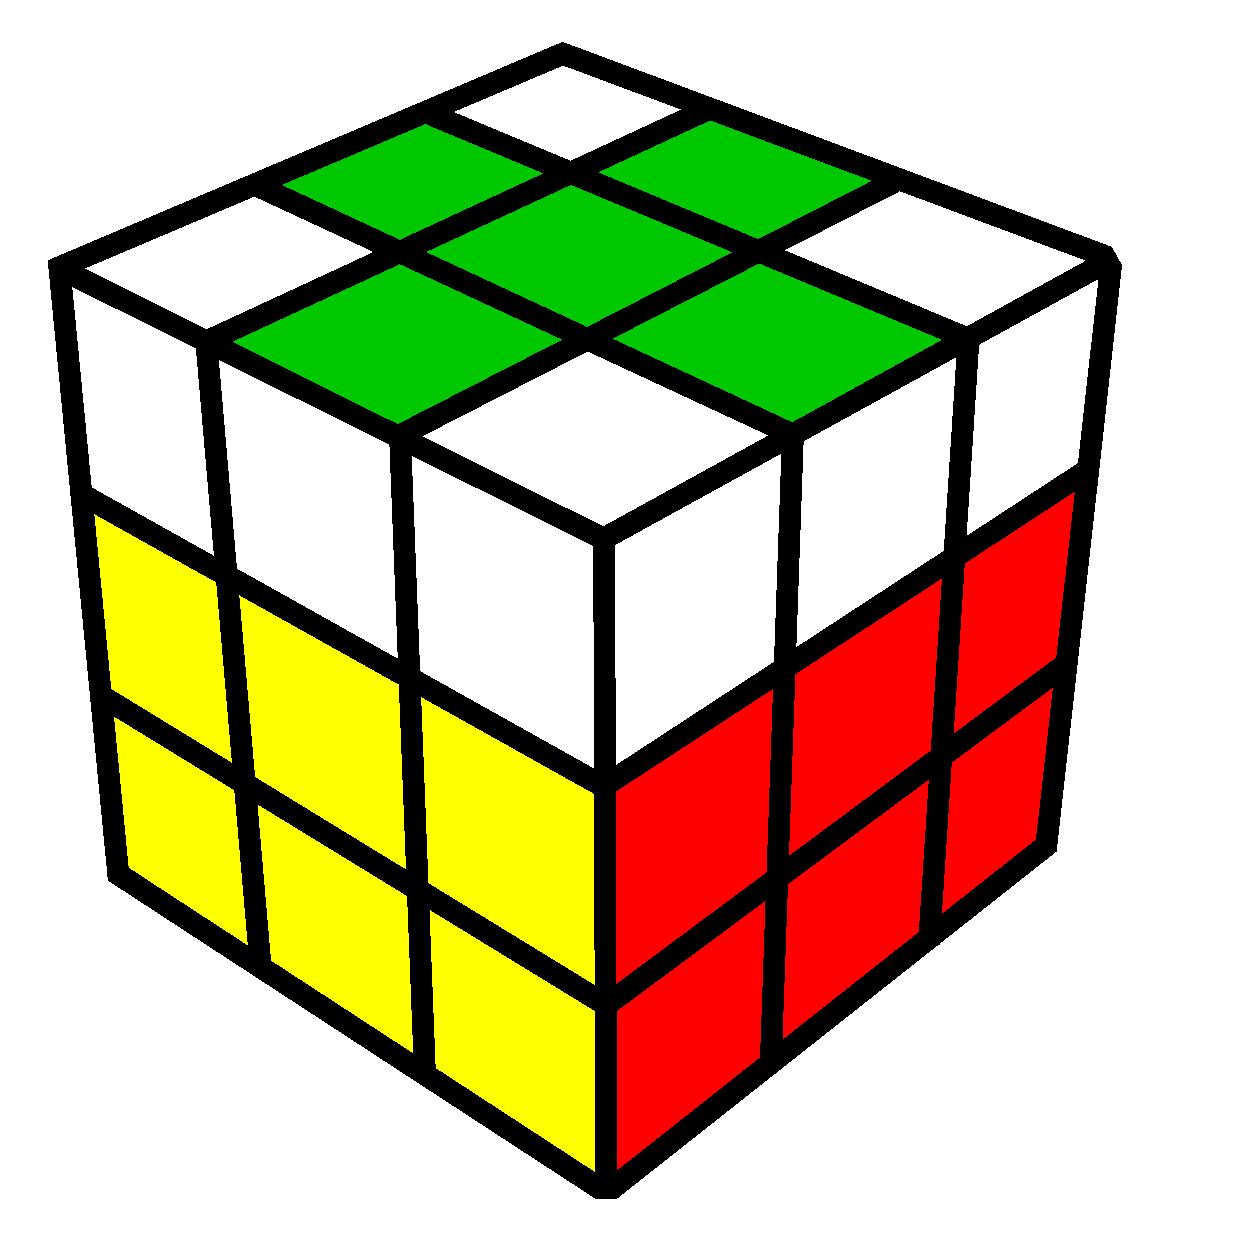
\includegraphics[scale=0.3]{img/layer3cross}}			
		\end{column}
		\begin{column}[C]{.5\textwidth}
			\begin{block}{Ziel}
				Ein Kreuz aus Steinen der Farbe oder Oberseite.
			\end{block}
			\begin{exampleblock}{Algorithmus}
				$FRUR^{-1}U^{-1}F^{-1}$
			\end{exampleblock}
			\begin{alertblock}{Wichtig}
				Der Würfel muss so gehalten werden, dass sich die Reihe horizontal zum Betrachter befindet.
			\end{alertblock}
		\end{column}
	\end{columns}
	
\end{frame}

\begin{frame}
	\frametitle{Wieder Kanten ausrichten}
	
	\begin{columns}[c]
		\begin{column}[C]{.5\textwidth}
			\center
			\only<1>{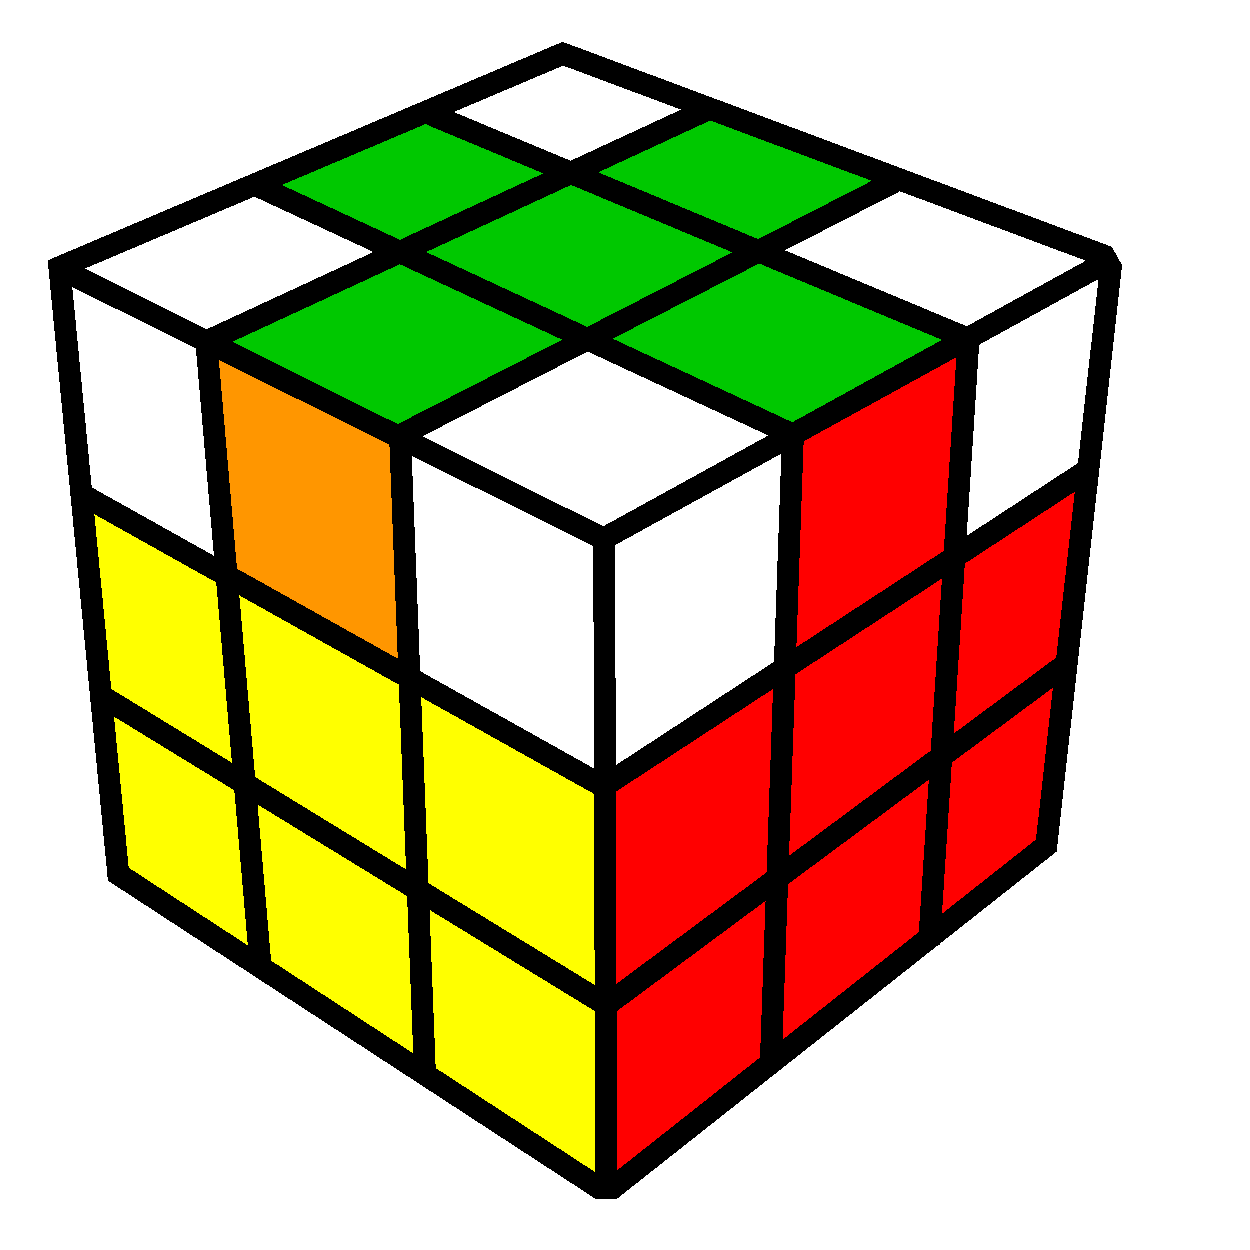
\includegraphics[scale=0.3]{img/layer3nodes1}}
			\only<2>{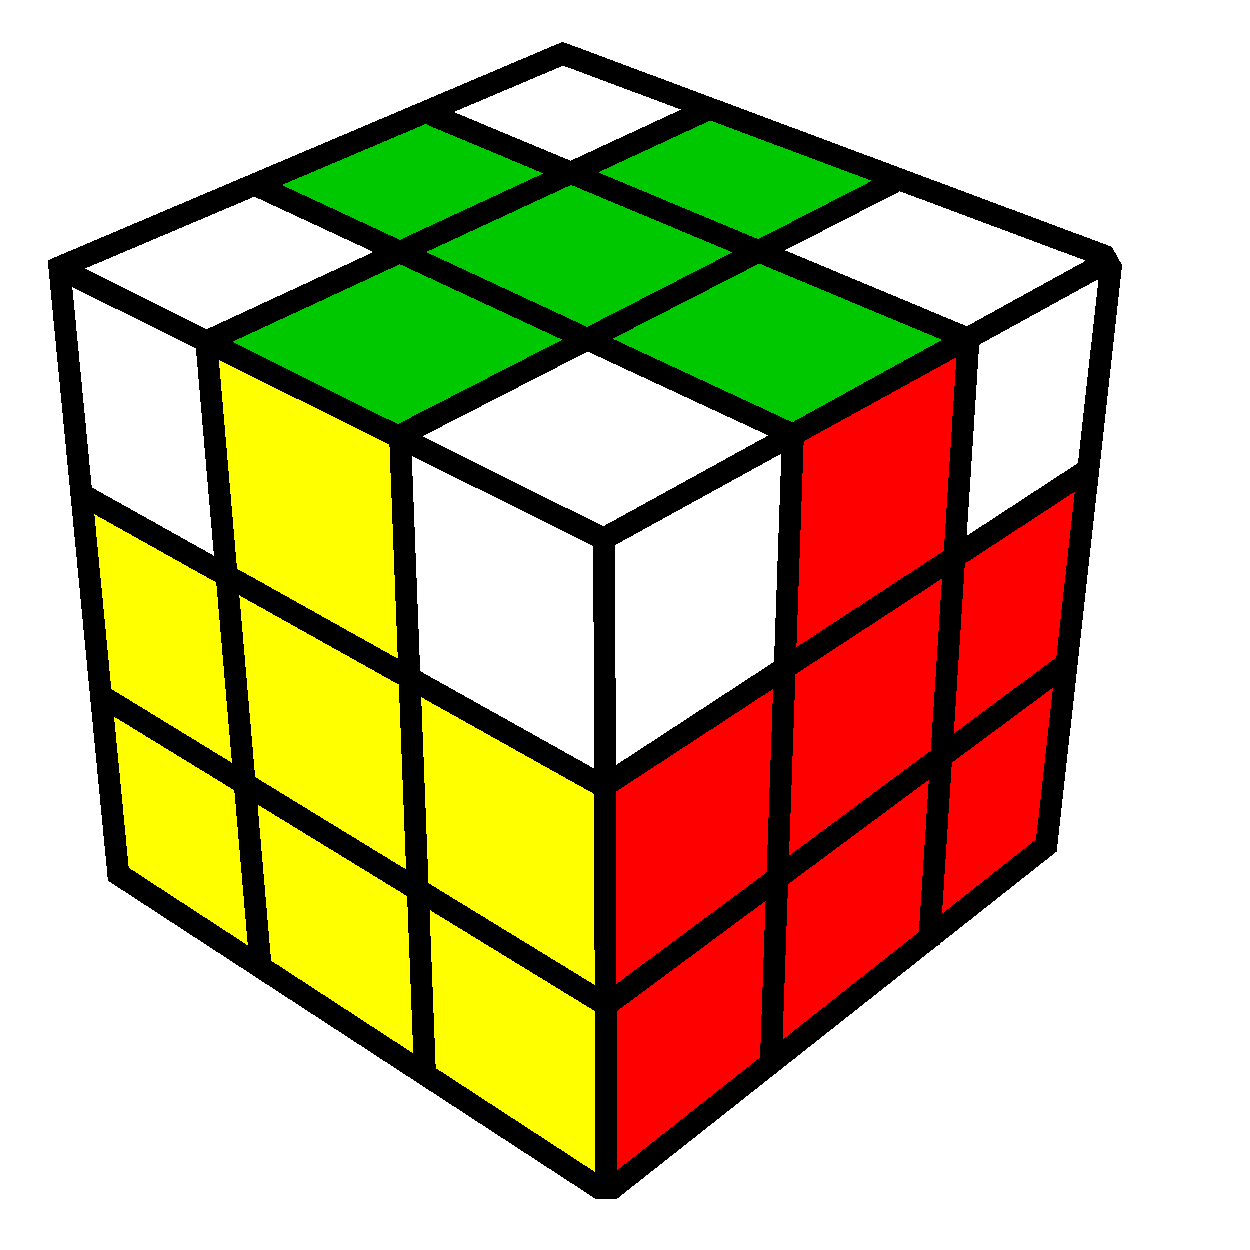
\includegraphics[scale=0.3]{img/layer3nodes2}}			
		\end{column}
		\begin{column}[C]{.5\textwidth}
			\begin{block}{Ziel}
				Die Kanten der Mittelstücke auf die jeweils richtige Seite bringen.
			\end{block}
			\begin{exampleblock}{Algorithmus}
				$RUR^{-1}URU^2R^{-1}U$
			\end{exampleblock}
			\begin{alertblock}{Wichtig}
				Es sind zuerst durch Drehen der Ebene 3 zwei passende Mittelstücke zu finden, der Würfel muss so gehalten werden dass sich diese rechts und hinten befinden.
			\end{alertblock}
		\end{column}
	\end{columns}
	
\end{frame}

\begin{frame}
	\frametitle{Wieder Ecken positionieren}
	
	\begin{columns}[c]
		\begin{column}[C]{.5\textwidth}
			\center
			\only<1>{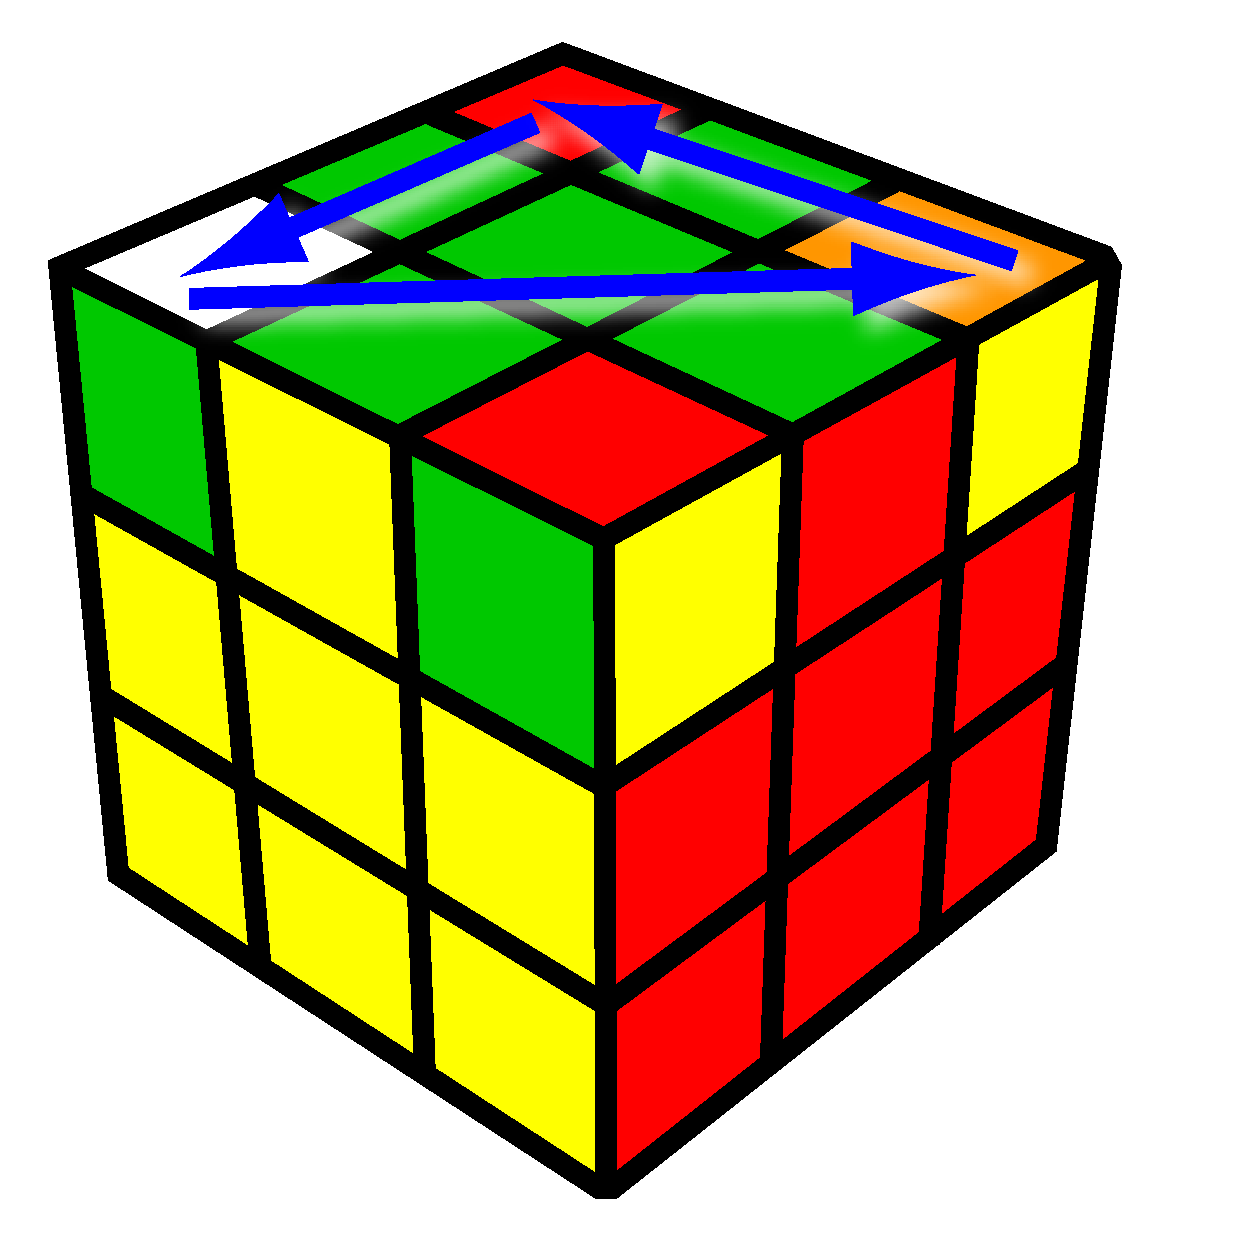
\includegraphics[scale=0.3]{img/layer3edges1}}
			\only<2>{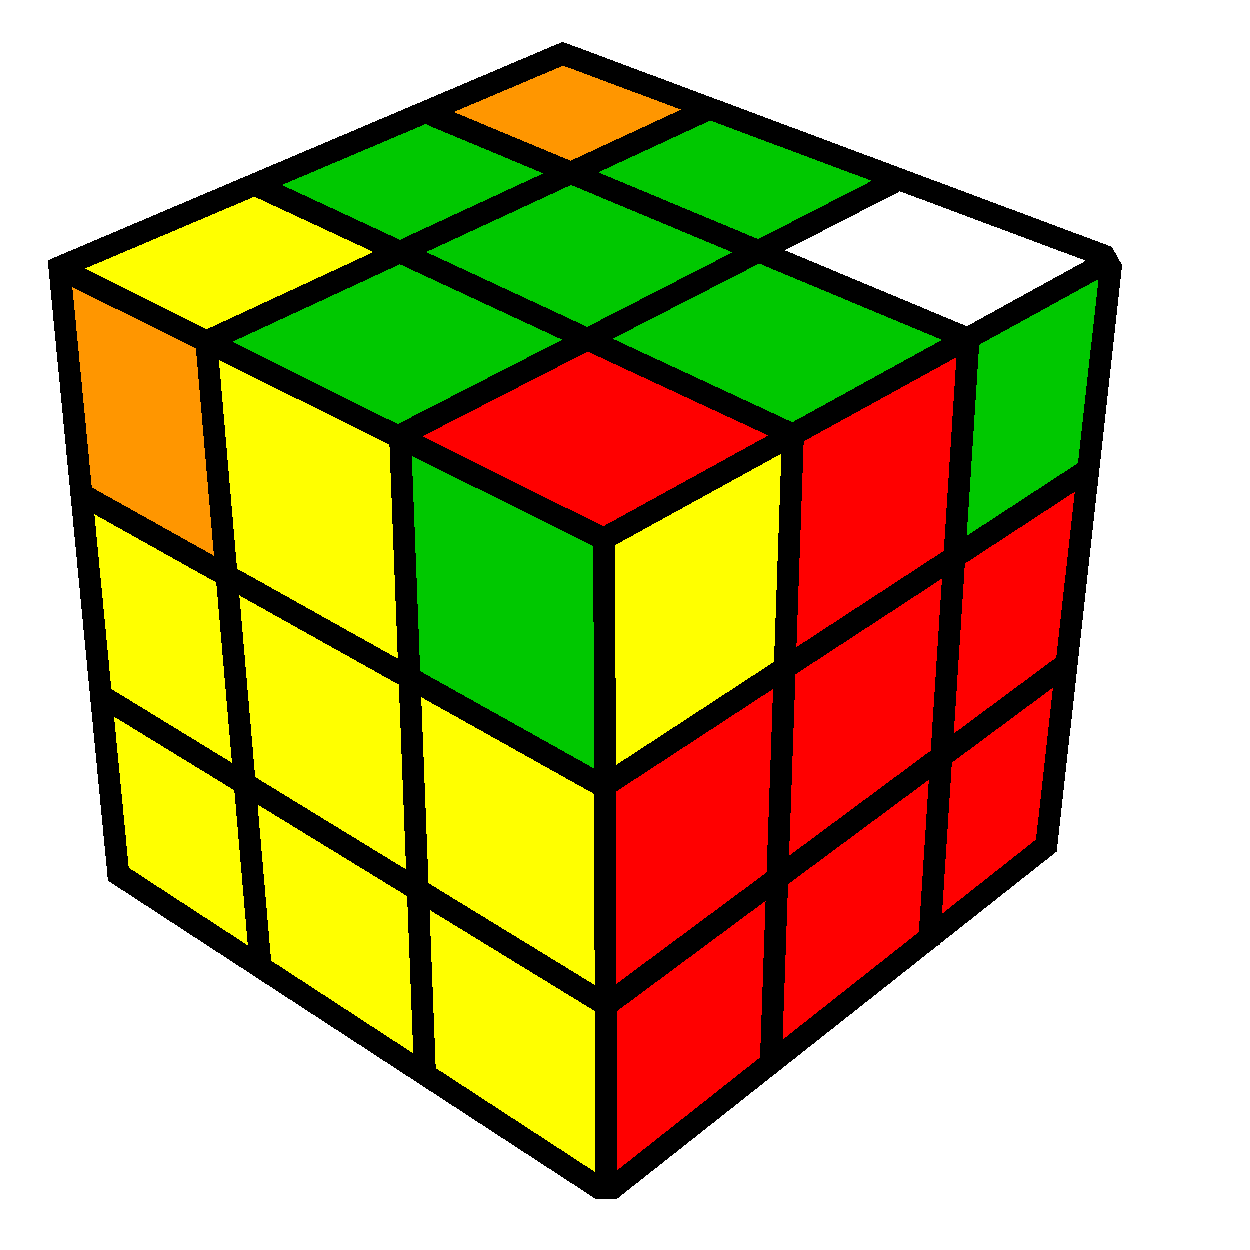
\includegraphics[scale=0.3]{img/layer3edges2}}
		\end{column}
		\begin{column}[C]{.5\textwidth}
			\begin{block}{Ziel}
				Die Ecken der Ebene 3 an die richtige Stelle bringen.
			\end{block}
			\begin{exampleblock}{Algorithmus}
				$URU^{-1}L^{-1}UR^{-1}U^{-1}L$
			\end{exampleblock}
			\begin{alertblock}{Wichtig}
				Eine Ecke befindet sich meist schon an der richtigen Stelle, diese muss dann \glqq vorne rechts\grqq{} gehalten werden.
			\end{alertblock}
		\end{column}
	\end{columns}
	
\end{frame}

\begin{frame}
	\frametitle{Wieder Ecken drehen}
	
	\begin{columns}[c]
		\begin{column}[C]{.5\textwidth}
			\center
			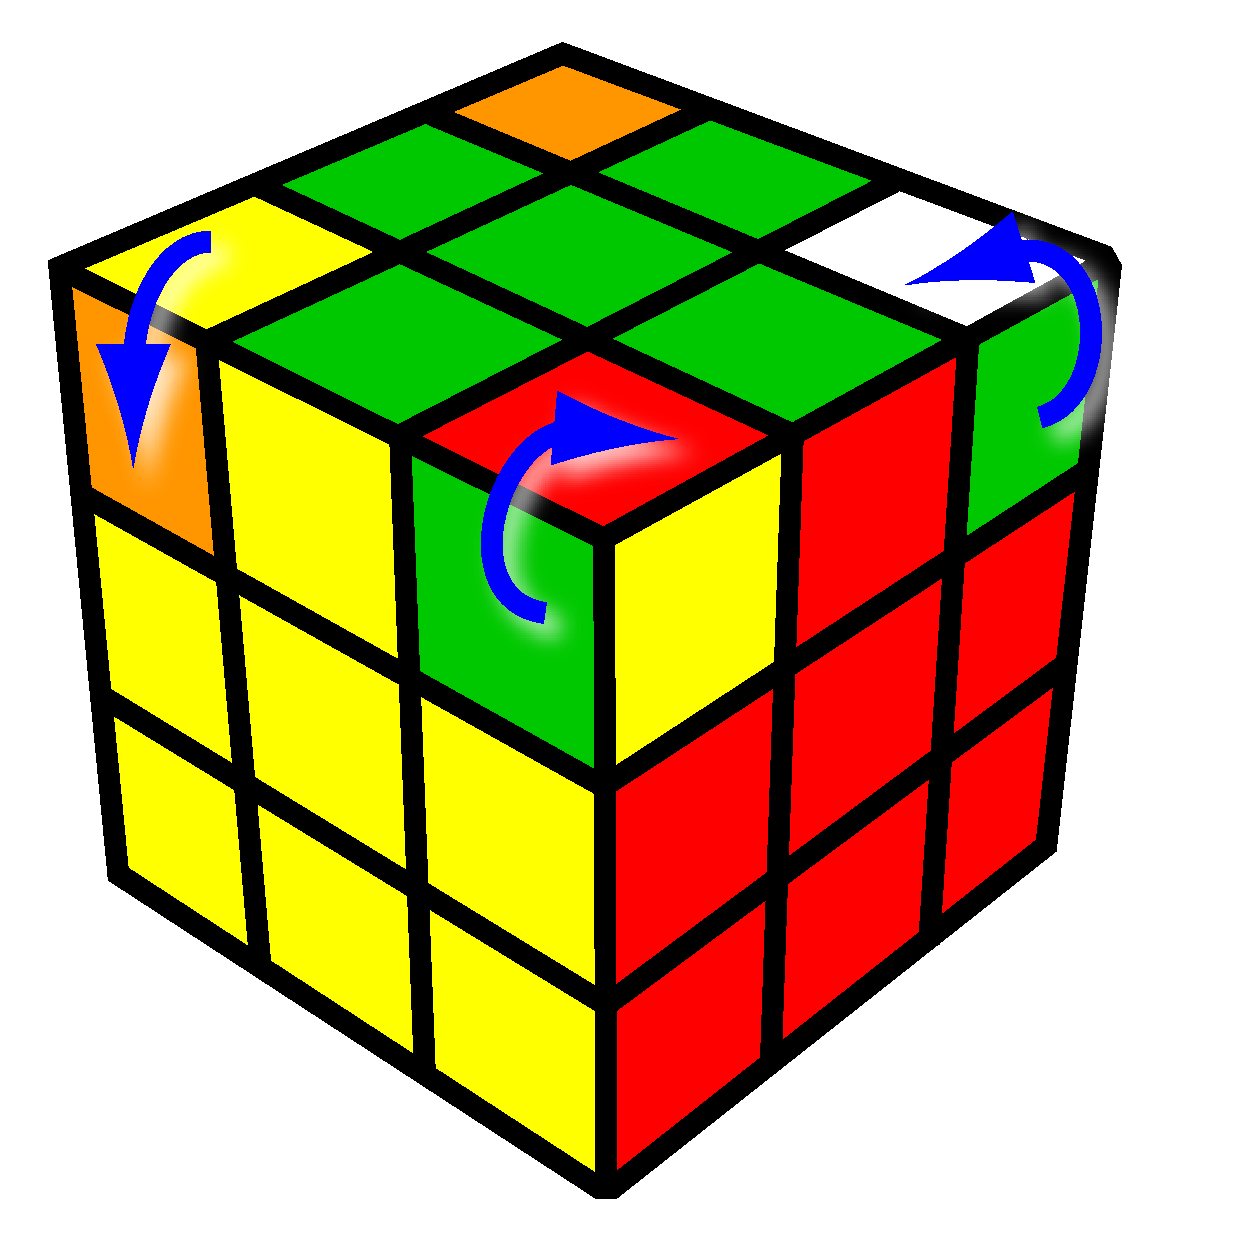
\includegraphics[scale=0.3]{img/layer3edges3}
		\end{column}
		\begin{column}[C]{.5\textwidth}
			\begin{block}{Ziel}
				Die Ecken der Ebene 3 richtig drehen.
			\end{block}
			\begin{exampleblock}{Algorithmus}
				$R^{-1}D^{-1}RD$
			\end{exampleblock}
			\begin{alertblock}{Wichtig}
				Wenn eine Ecke richtig gedreht ist, die Ebene 3 um 90\gradneu{} im Uhrzeigersinn drehen und die nächste Ecke bearbeiten.
			\end{alertblock}
		\end{column}
	\end{columns}
	
\end{frame}

\begin{frame}
	\frametitle{Fertig!}
	
	\begin{columns}[c]
		\begin{column}[C]{.5\textwidth}
			\center
			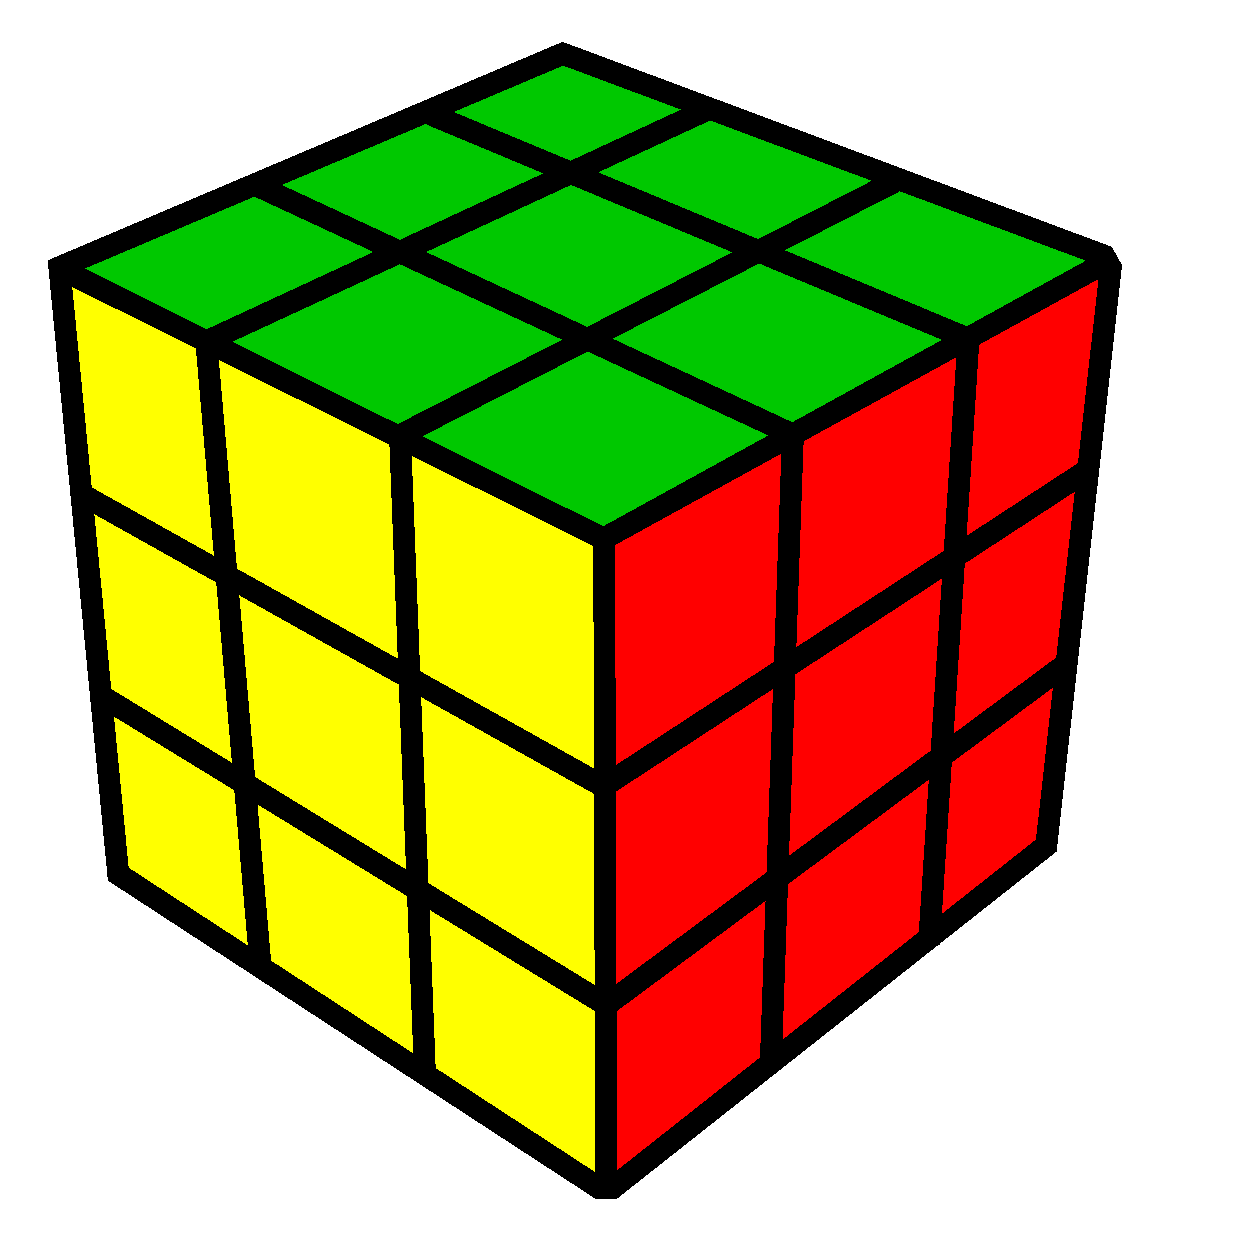
\includegraphics[scale=0.3]{img/solved3}
		\end{column}
		\begin{column}[C]{.5\textwidth}
			Herzlichen Glückwunsch, du hast gerade deinen Zauberwürfel gelöst!
		\end{column}
	\end{columns}
	
\end{frame}

% section ebene_3 (end)